% AL: This is an alternate version of Lecture 01 developed by Andre.
% It would be good to merge this into a single lecture. Some of the
% material here can be moved to Lecture 05.

\documentclass{fenicscourse}

\begin{document}

\fenicslecture{Lecture 1: Introduction to FEniCS}
              {Anders Logg\\
               Andr\'e Massing}

\fenicssection{What is FEniCS?}

\begin{frame}
  \frametitle{FEniCS is an automated programming environment for differential equations}
  \normalsize

  \begin{columns}

    \begin{column}{0.6\textwidth}

      \begin{itemize}
      \item
        C++/Python library
      \item
        Initiated 2003 in Chicago
      \item
        1000--2000 monthly downloads
      \item
        Part of Debian and Ubuntu
      \item
        Licensed under the GNU LGPL
      \end{itemize}

      \vspace{0.5cm}

      \large
      \texttt{http://fenicsproject.org/}

    \end{column}

    \begin{column}{0.4\textwidth}
      
\includegraphics[height=4cm]{png/fenics_logo.png}
    \end{column}

  \end{columns}

  \vspace{0.5cm}

  \begin{block}{Collaborators}
    \it
    Simula Research Laboratory,
    University of Cambridge,
    University of Chicago,
    Texas Tech University,
    KTH Royal Institute of Technology,
    Chalmers University of Technology,
    Imperial College London,
    University of Oxford,
    Charles University in Prague,
    \ldots
  \end{block}

\end{frame}

\begin{frame}
  \frametitle{FEniCS is automated FEM}

  \begin{itemize}
  \item
    Automated generation of basis functions
  \item
    Automated evaluation of variational forms
  \item
    Automated finite element assembly
  \item
    Automated adaptive error control
  \end{itemize}

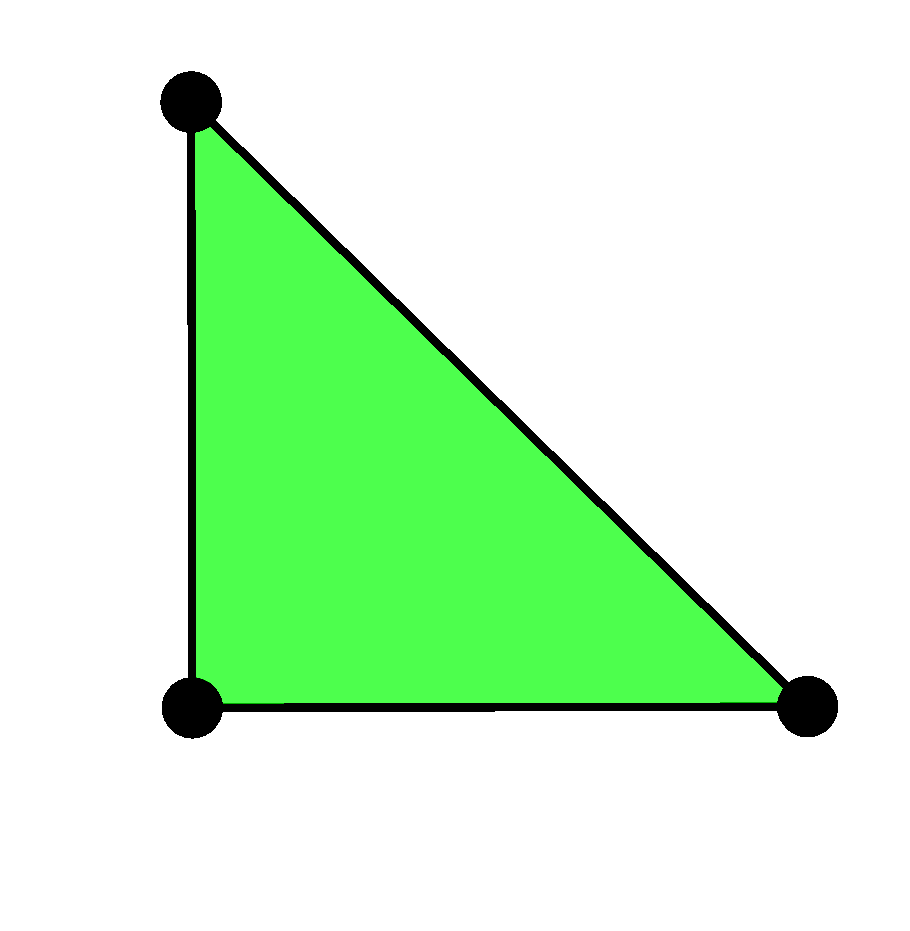
\includegraphics[width=1.3cm]{png/CG1_2d.png}
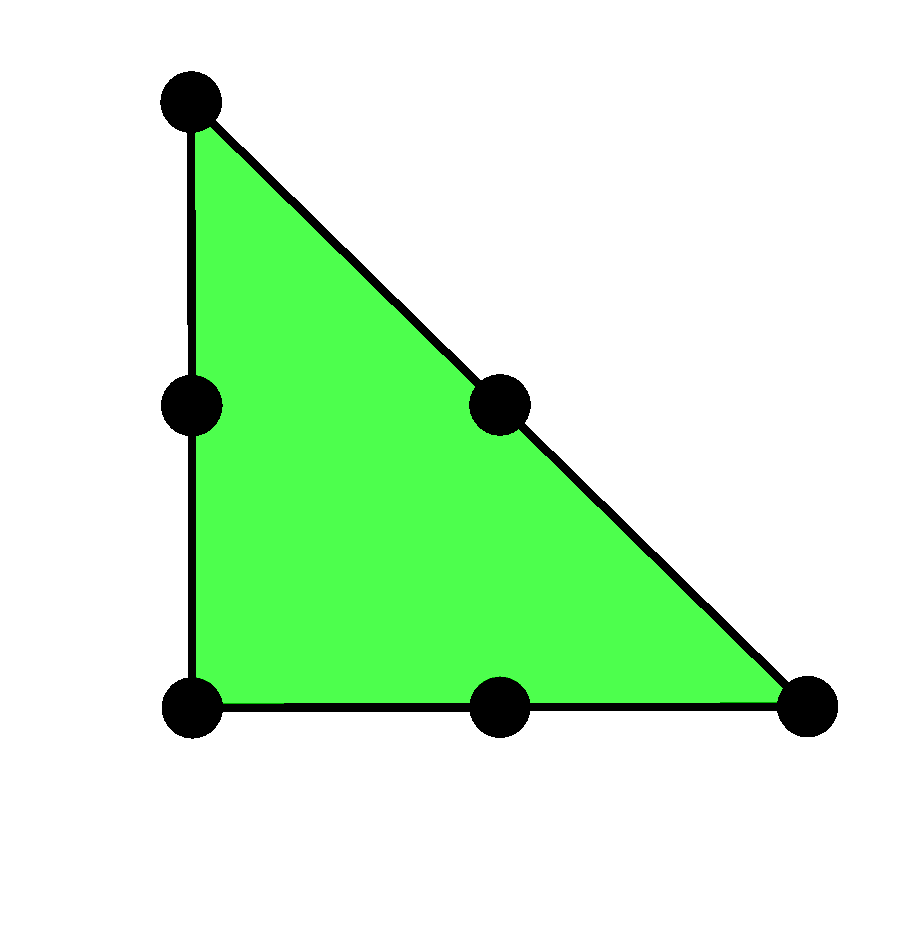
\includegraphics[width=1.3cm]{png/CG2_2d.png}
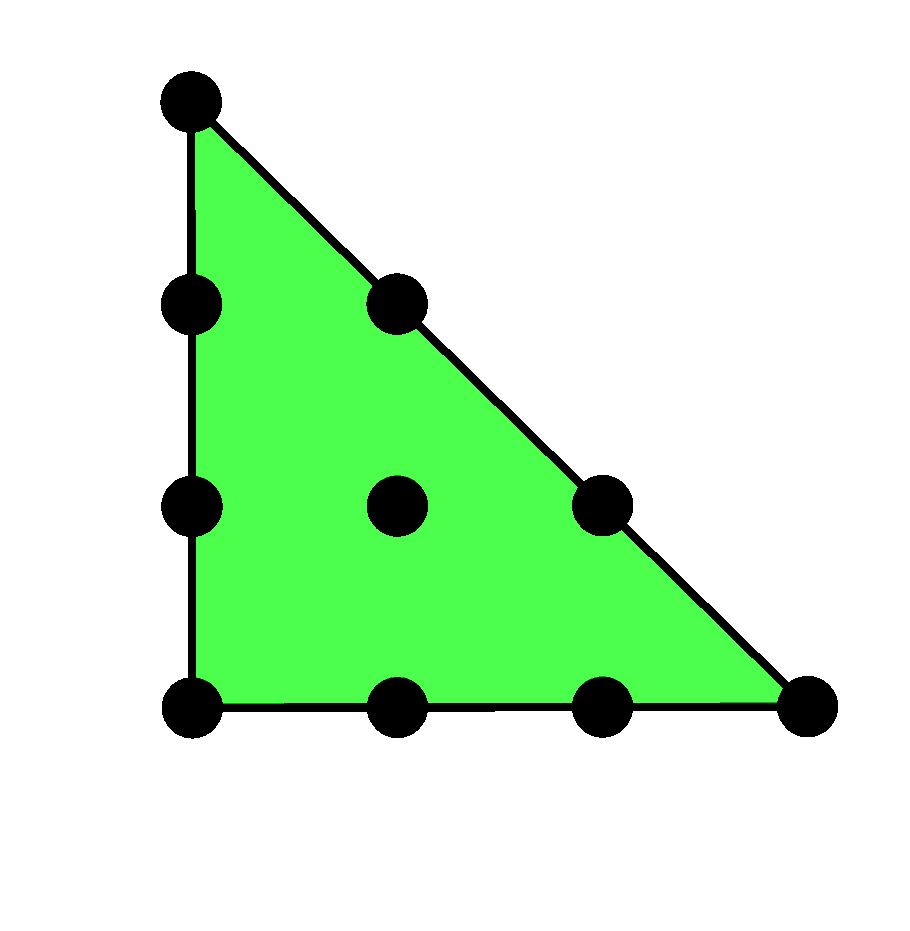
\includegraphics[width=1.3cm]{png/CG3_2d.png}
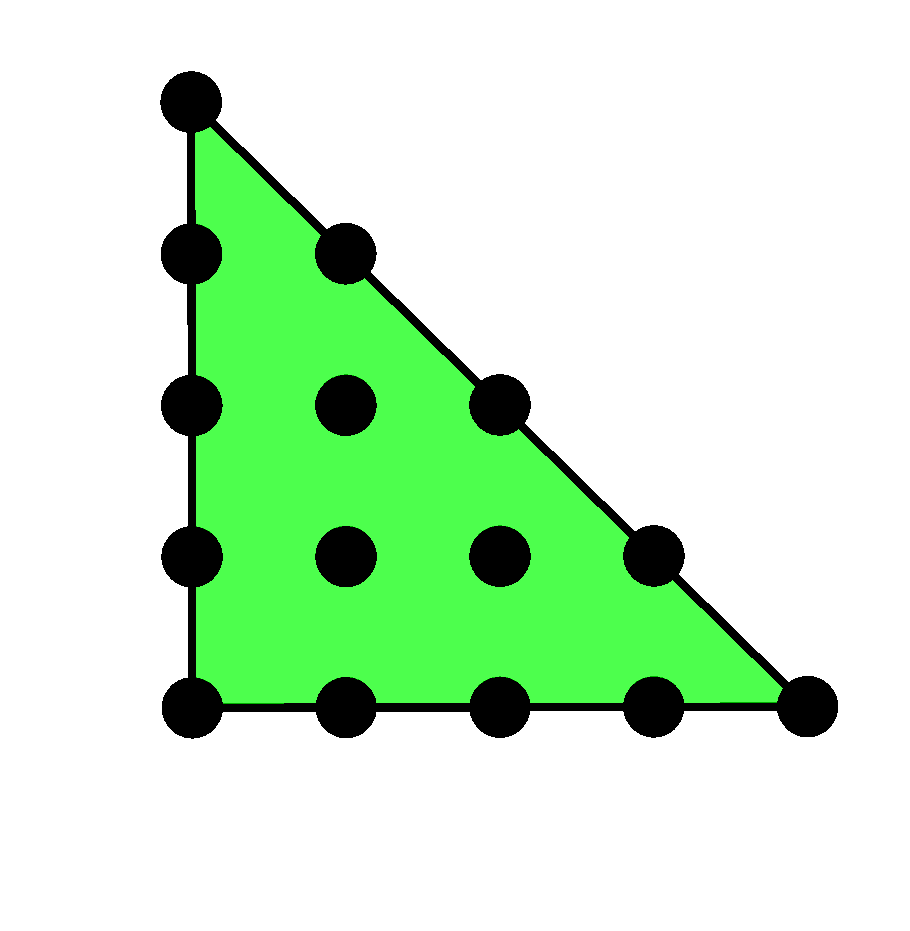
\includegraphics[width=1.3cm]{png/CG4_2d.png}
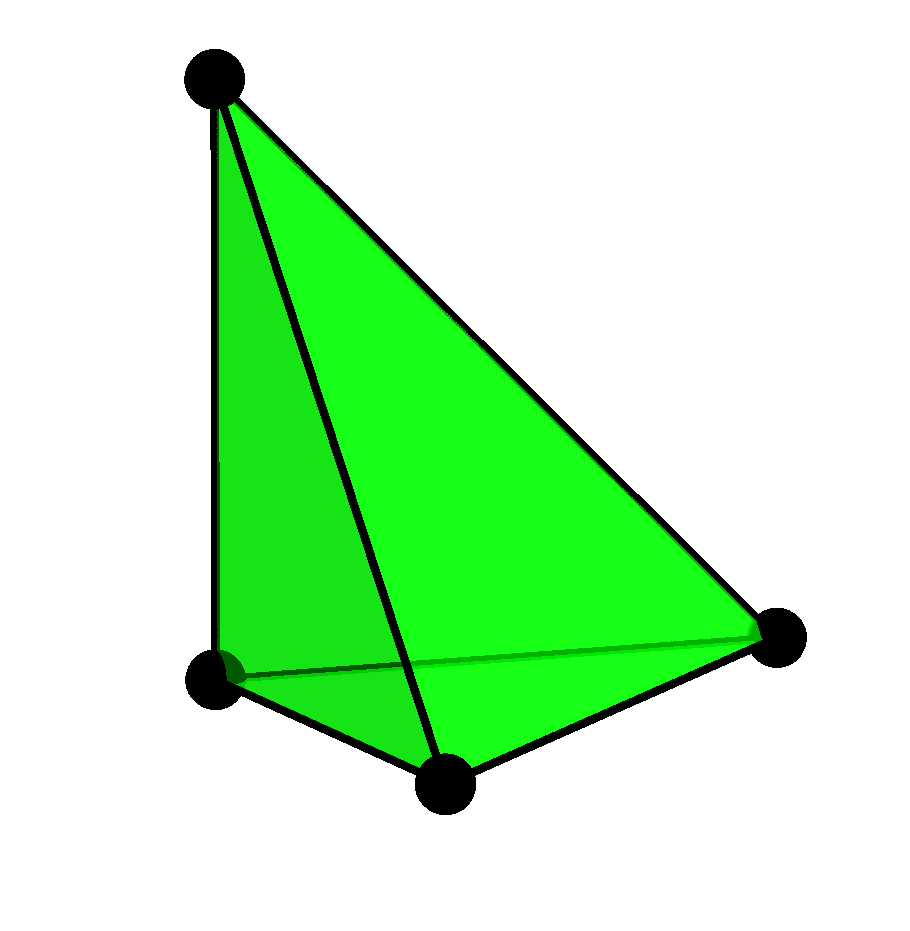
\includegraphics[width=1.3cm]{png/CG1_3d.png}
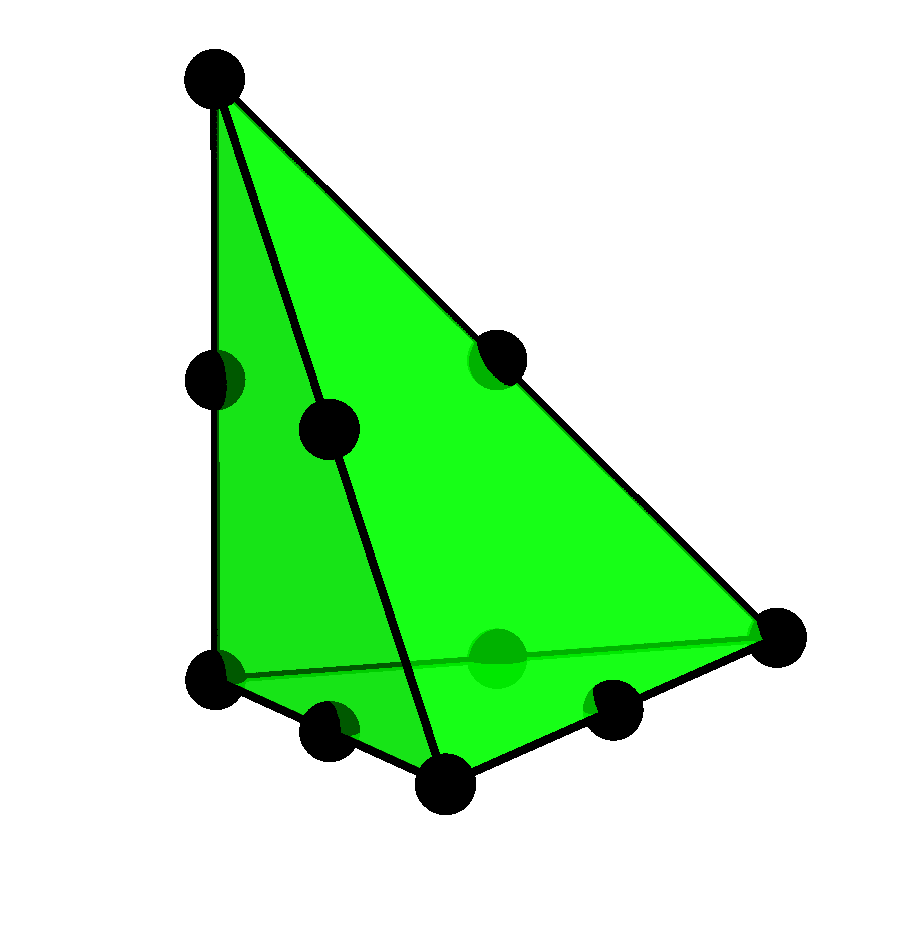
\includegraphics[width=1.3cm]{png/CG2_3d.png}
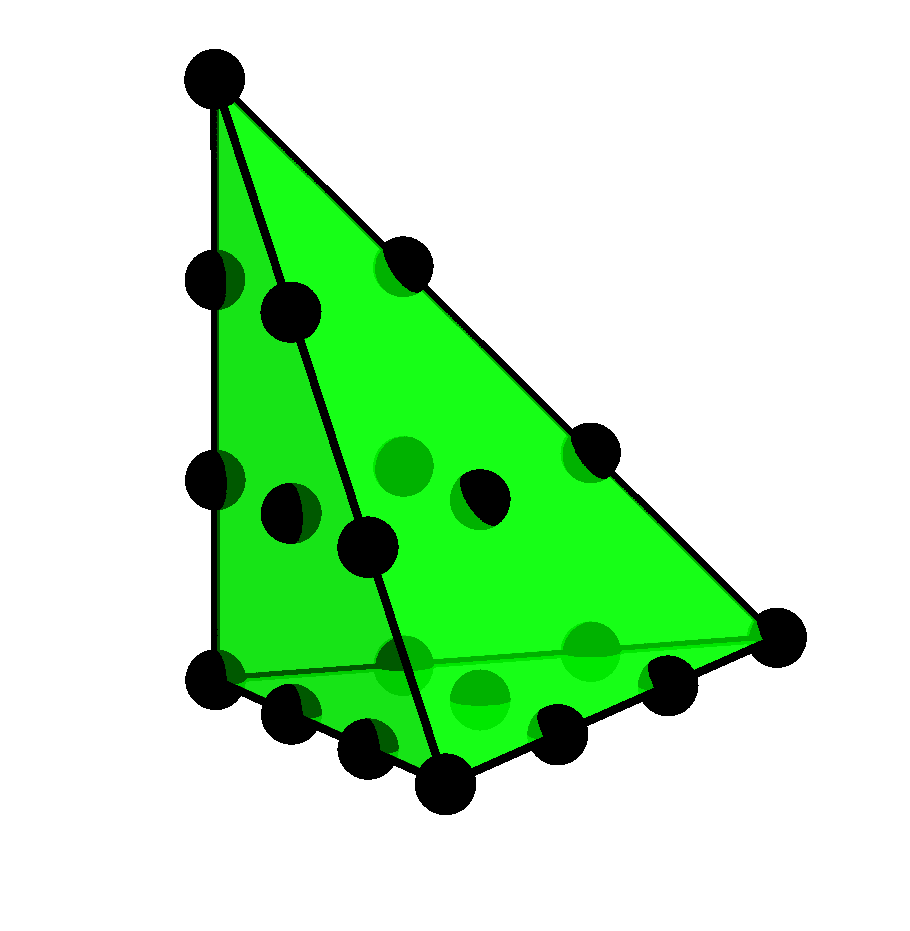
\includegraphics[width=1.3cm]{png/CG3_3d.png}
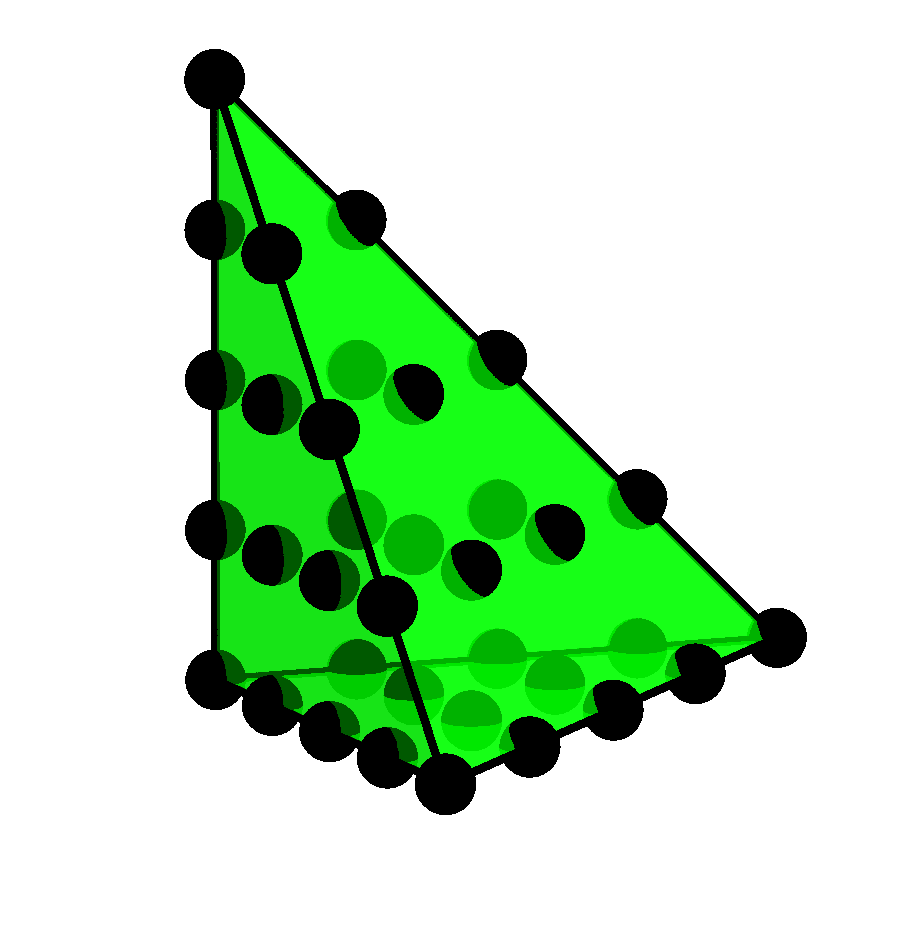
\includegraphics[width=1.3cm]{png/CG4_3d.png} \\
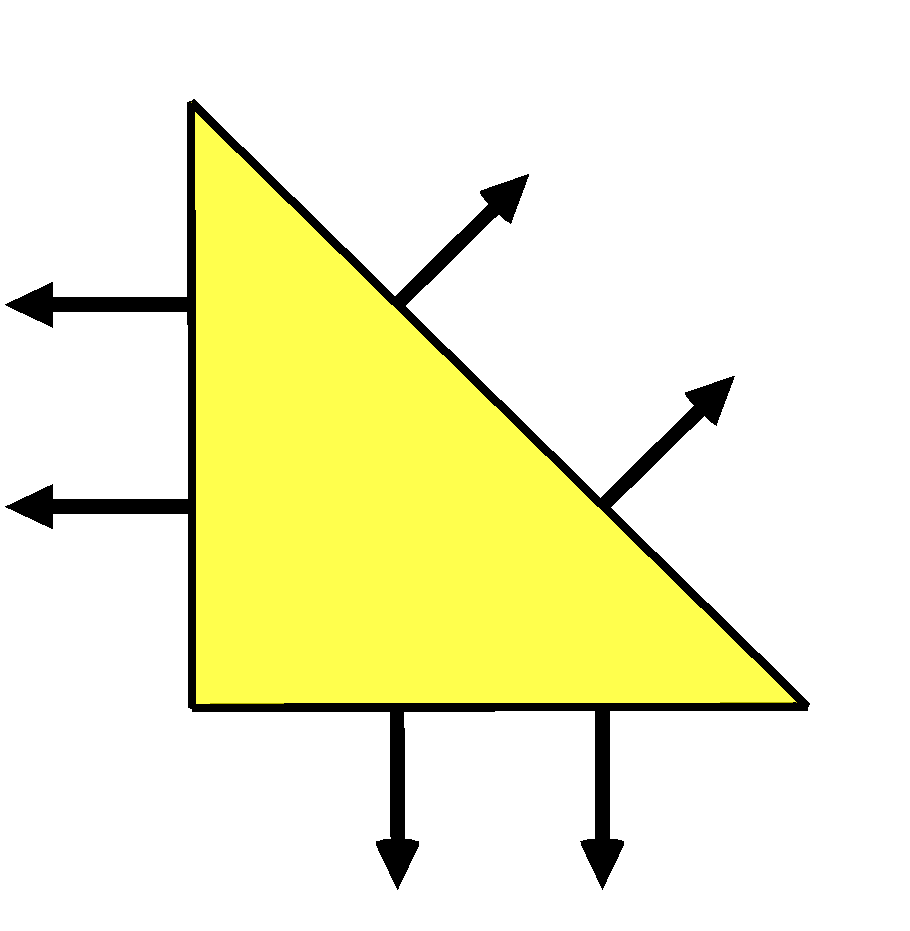
\includegraphics[width=1.3cm]{png/BDM1_2d.png}
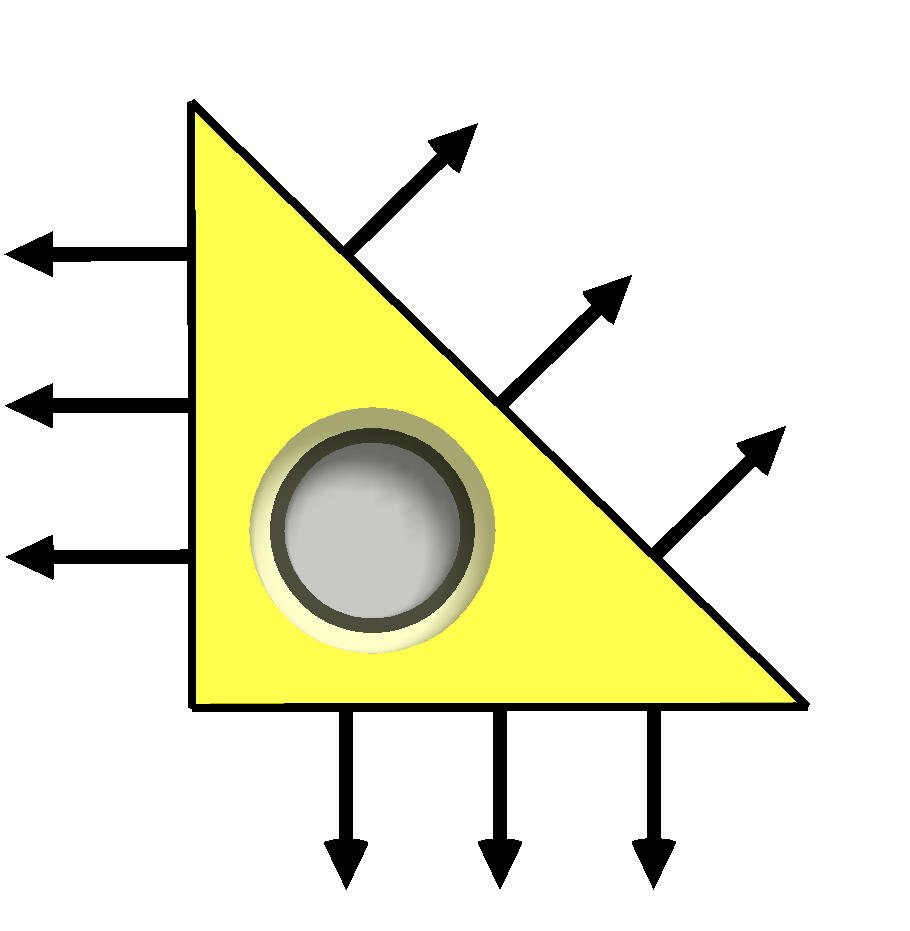
\includegraphics[width=1.3cm]{png/BDM2_2d.png}
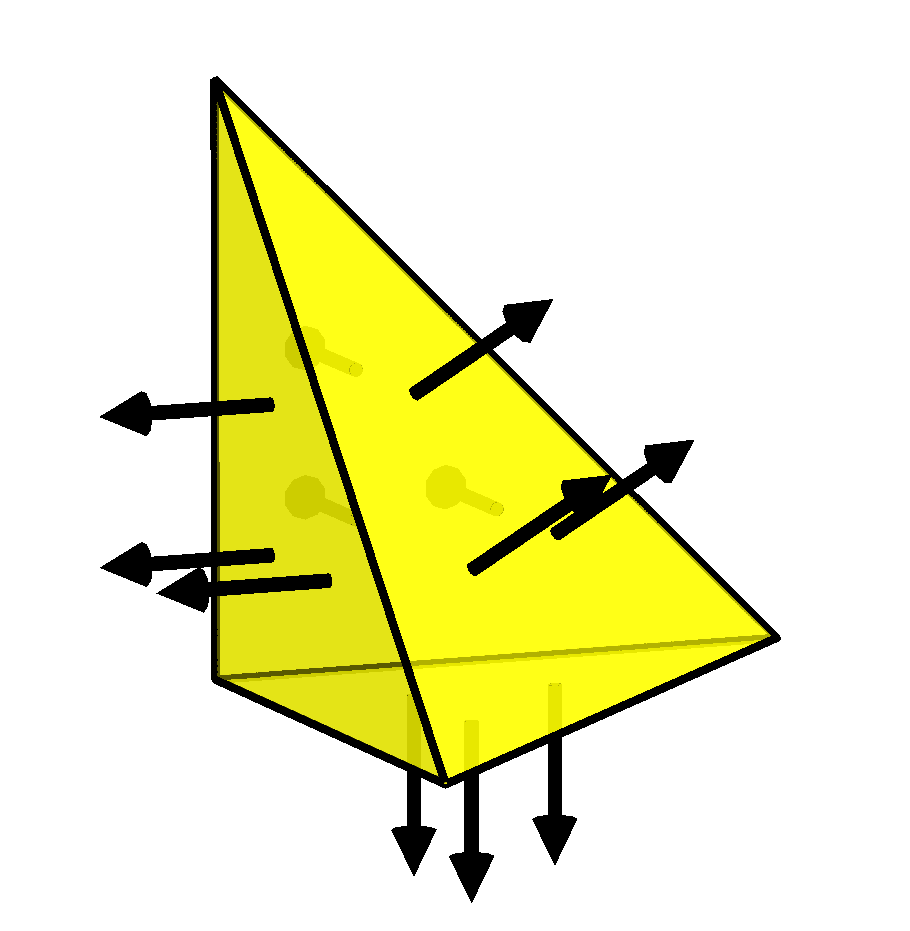
\includegraphics[width=1.3cm]{png/BDM1_3d.png}
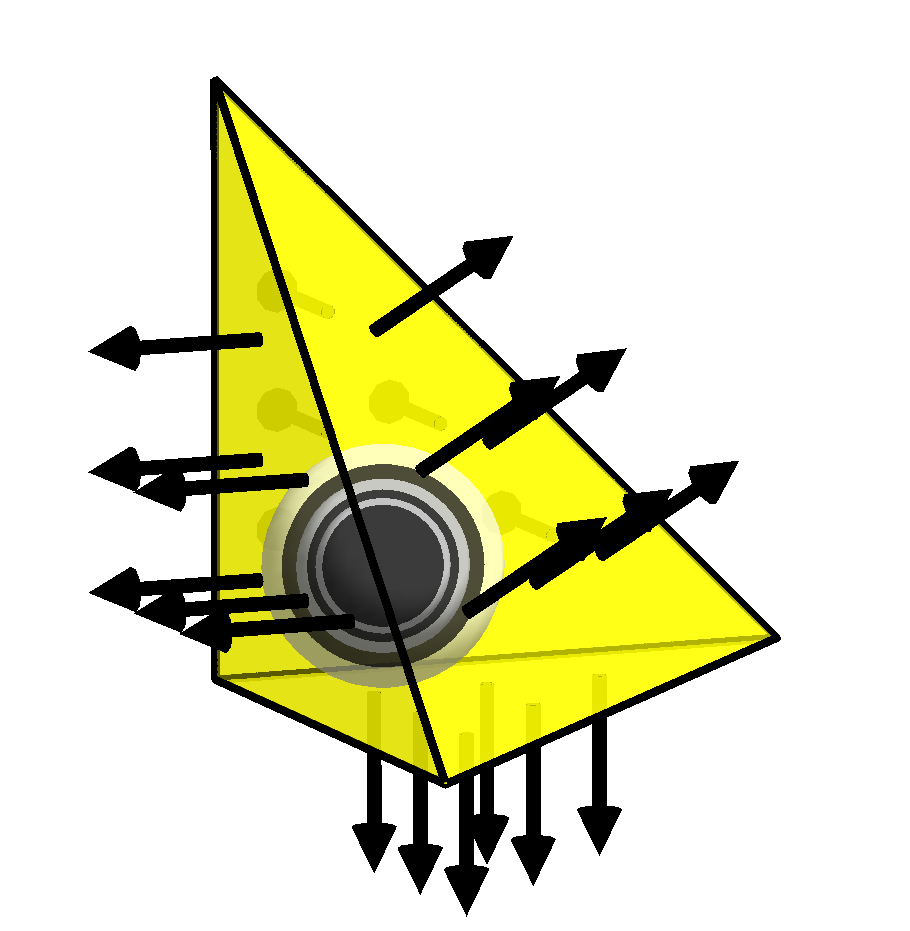
\includegraphics[width=1.3cm]{png/BDM2_3d.png}
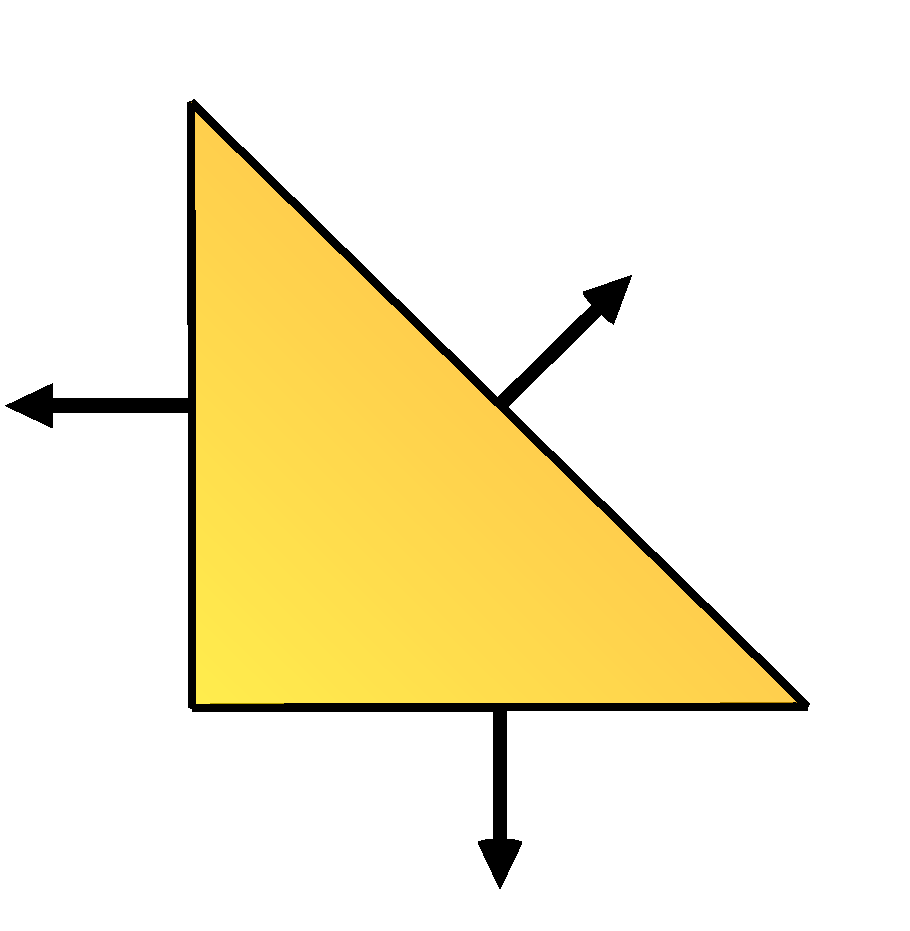
\includegraphics[width=1.3cm]{png/RT1_2d.png}
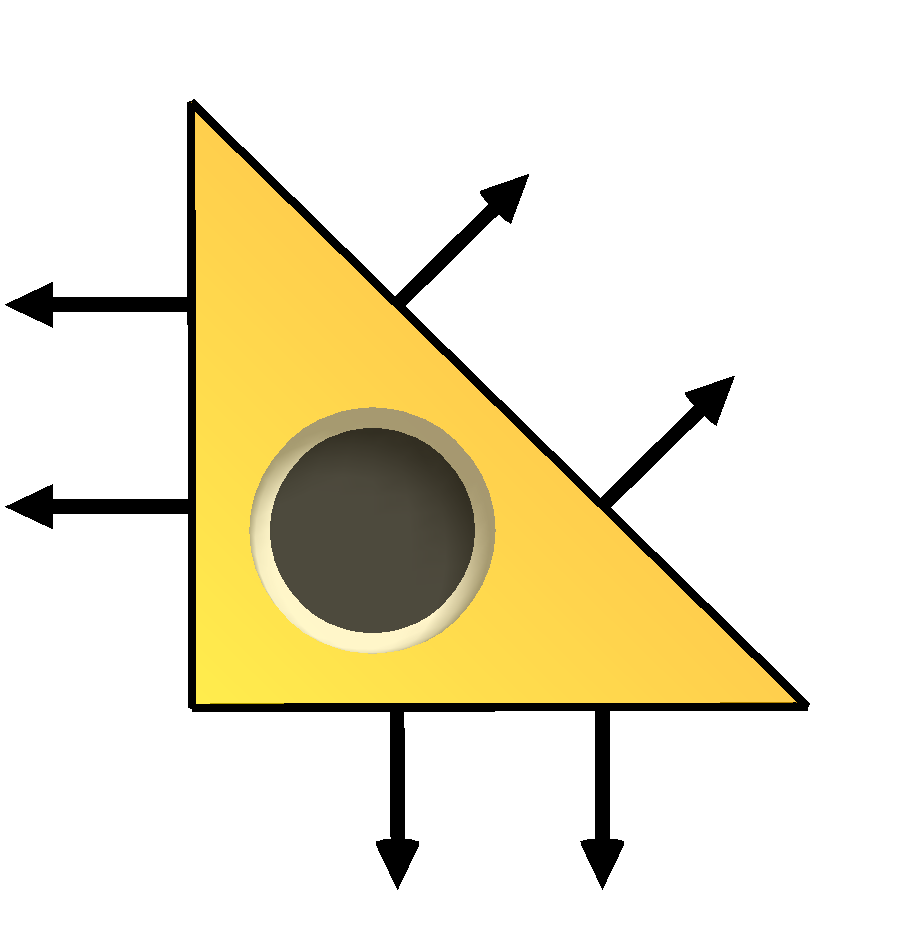
\includegraphics[width=1.3cm]{png/RT2_2d.png}
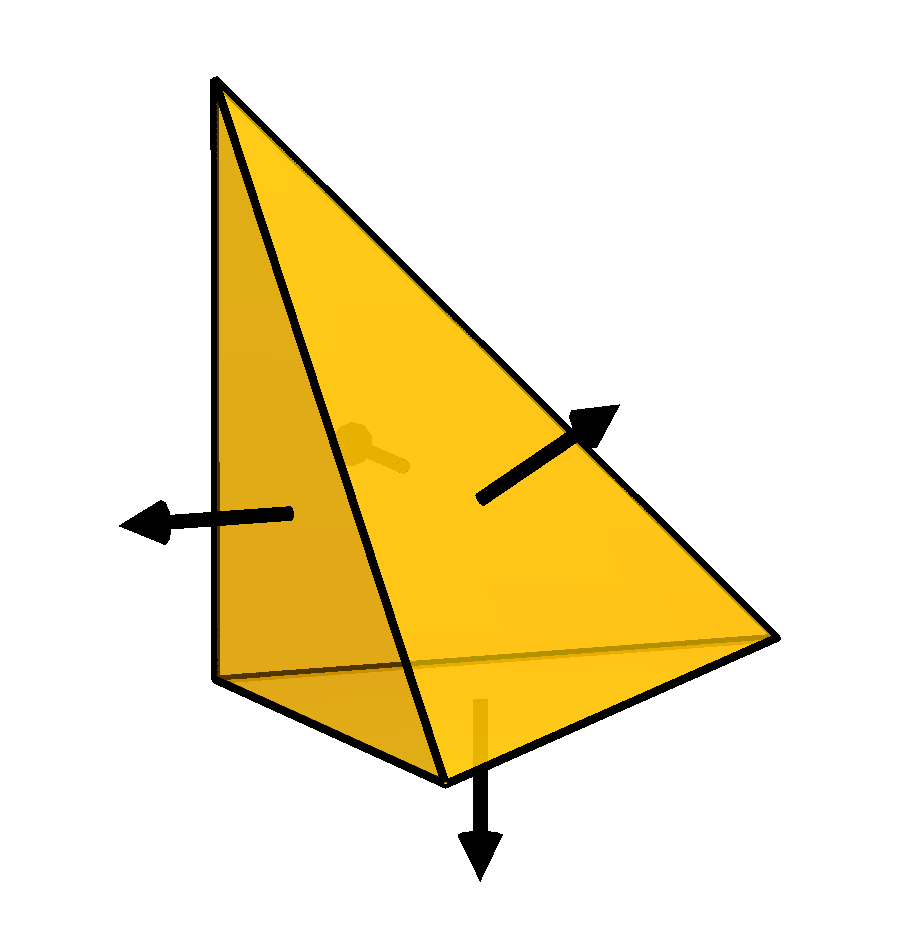
\includegraphics[width=1.3cm]{png/RT1_3d.png}
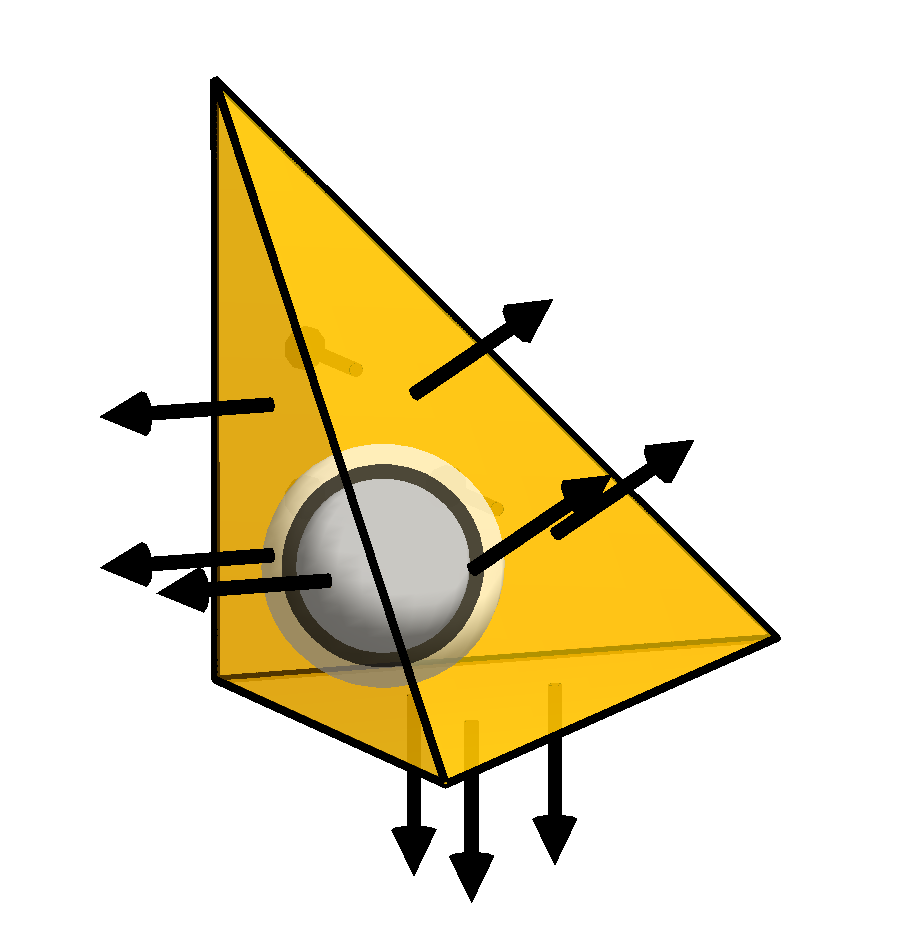
\includegraphics[width=1.3cm]{png/RT2_3d.png} \\
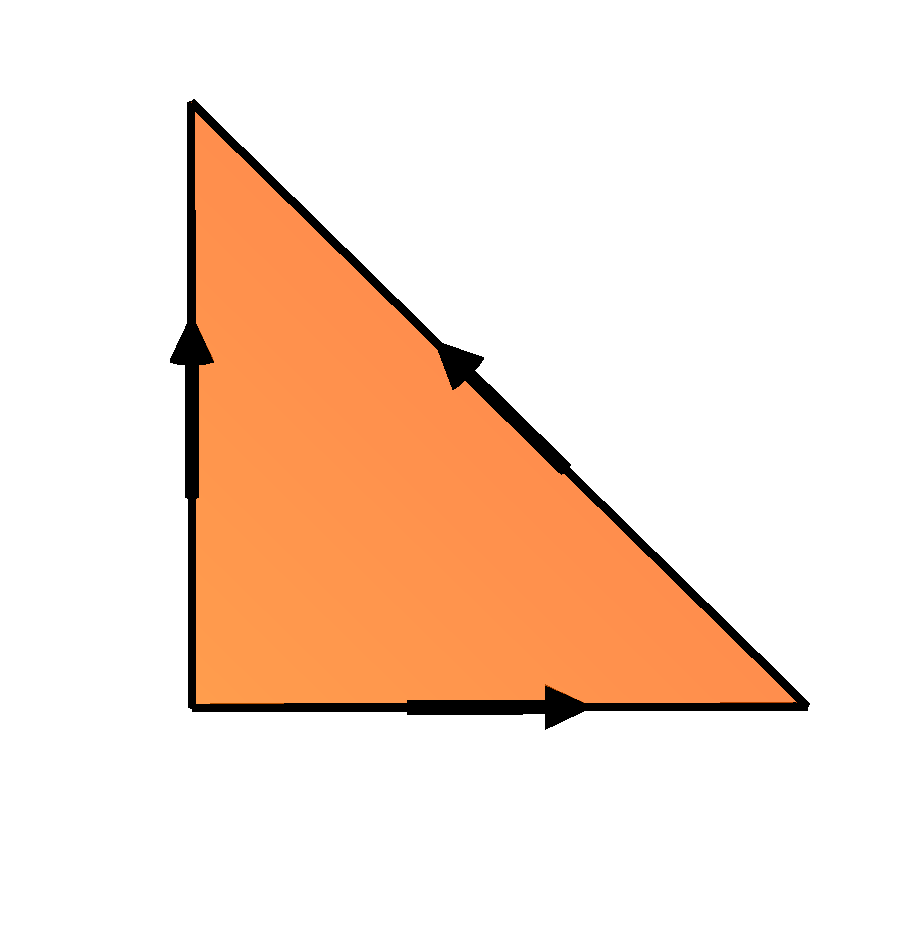
\includegraphics[width=1.3cm]{png/NED1_1_2d.png}
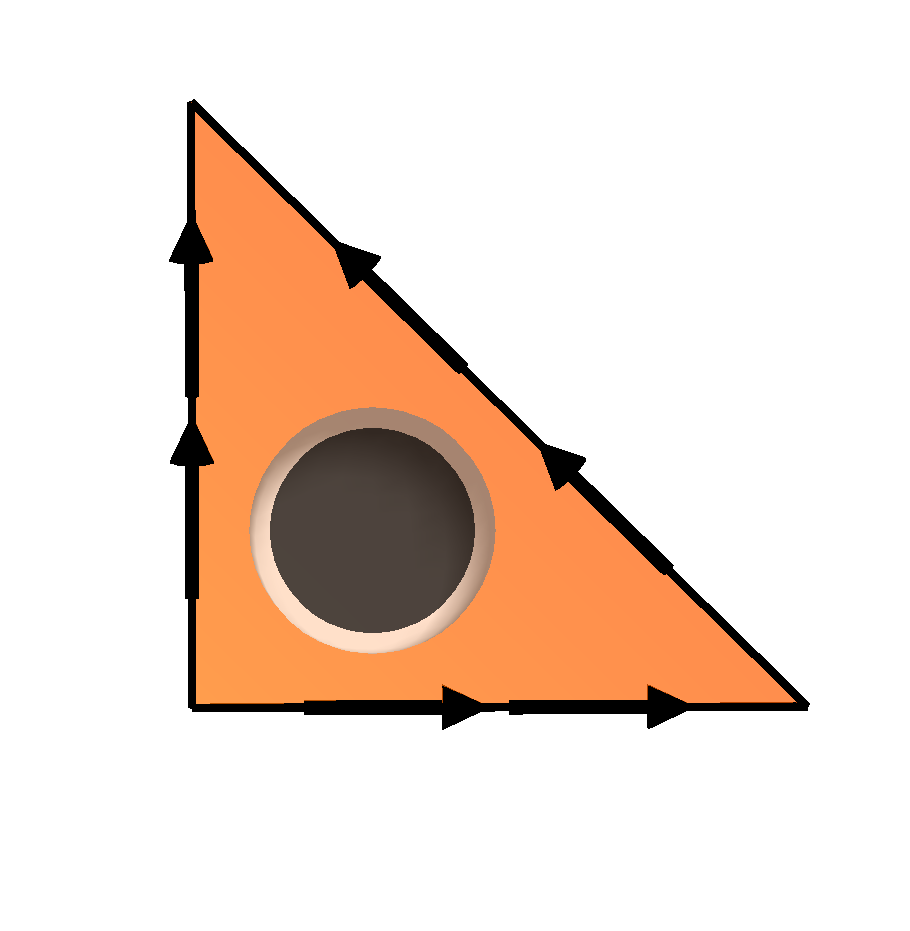
\includegraphics[width=1.3cm]{png/NED1_2_2d.png}
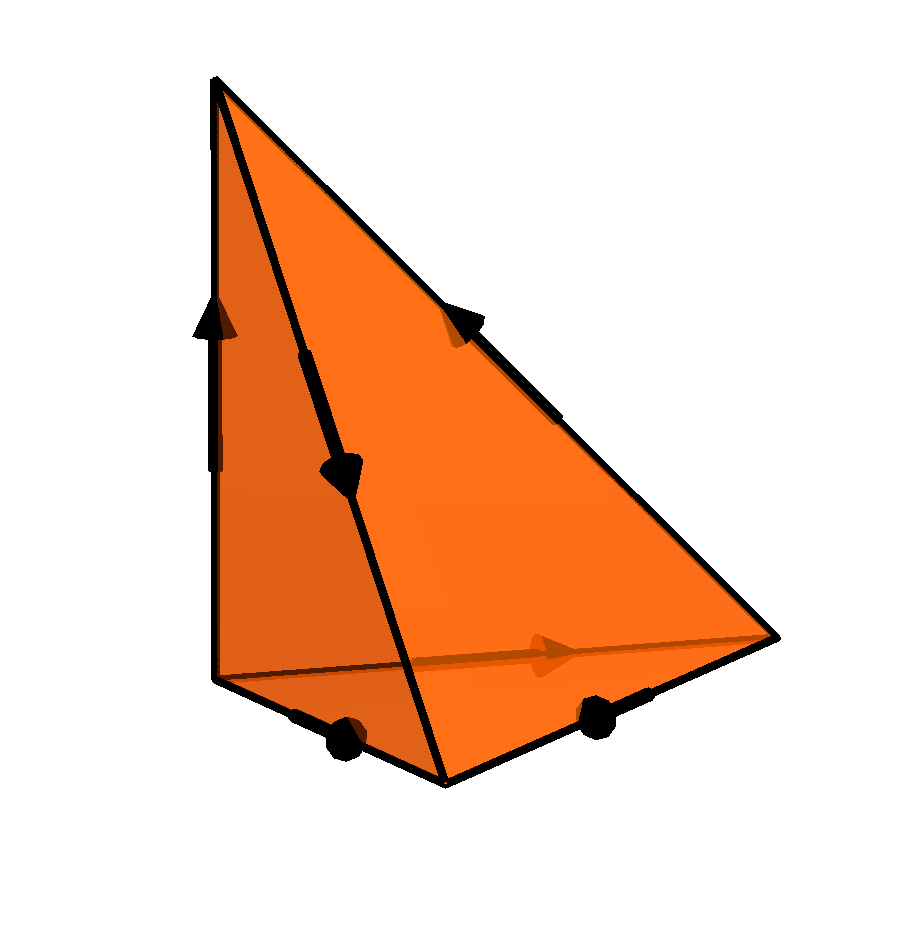
\includegraphics[width=1.3cm]{png/NED1_1_3d.png}
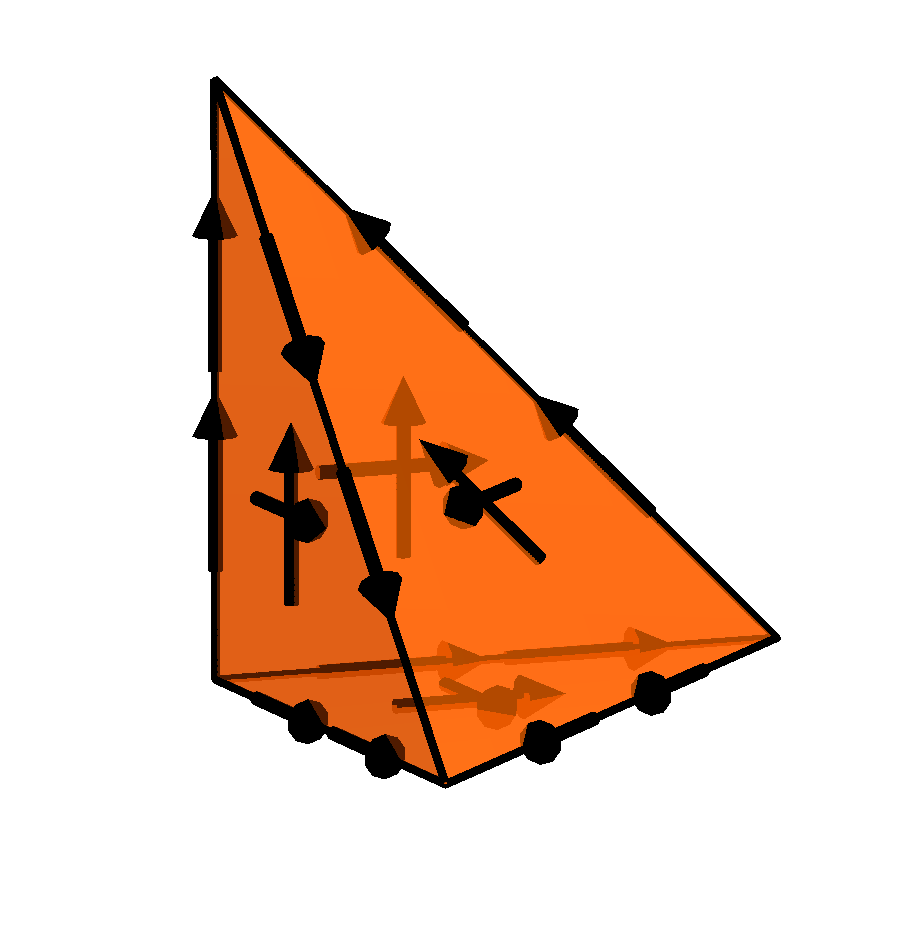
\includegraphics[width=1.3cm]{png/NED1_2_3d.png}
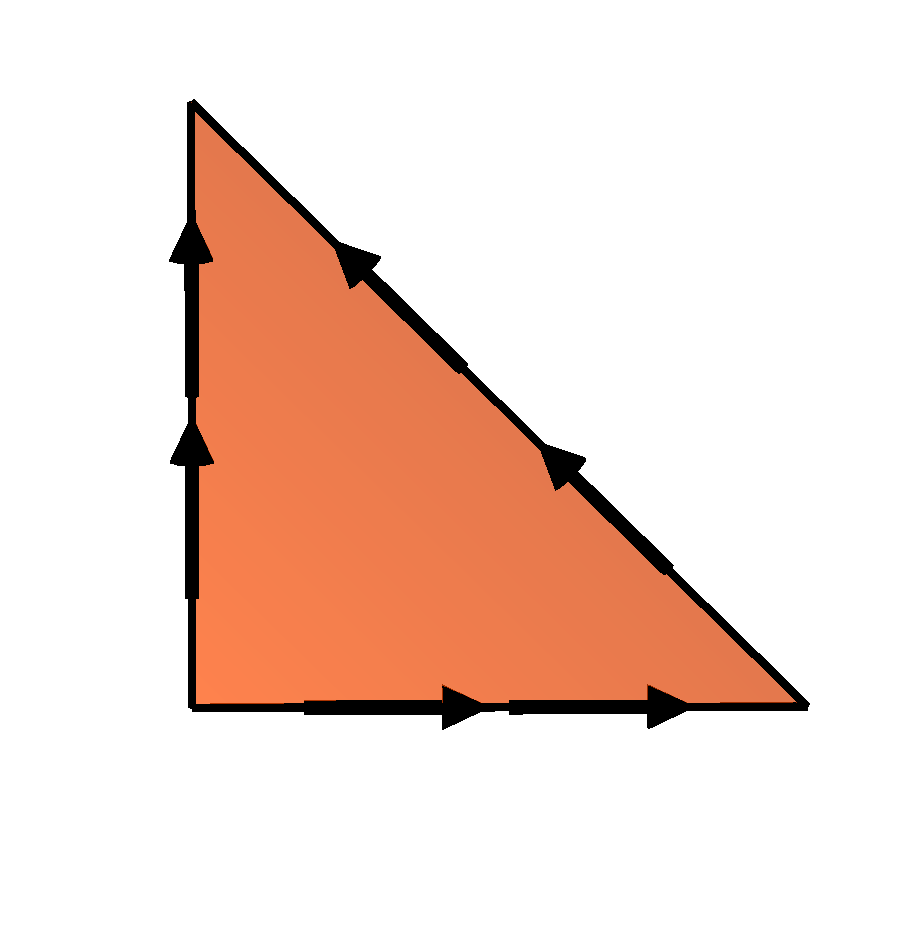
\includegraphics[width=1.3cm]{png/NED2_1_2d.png}

\includegraphics[width=1.3cm]{png/NED2_2_2d.png}
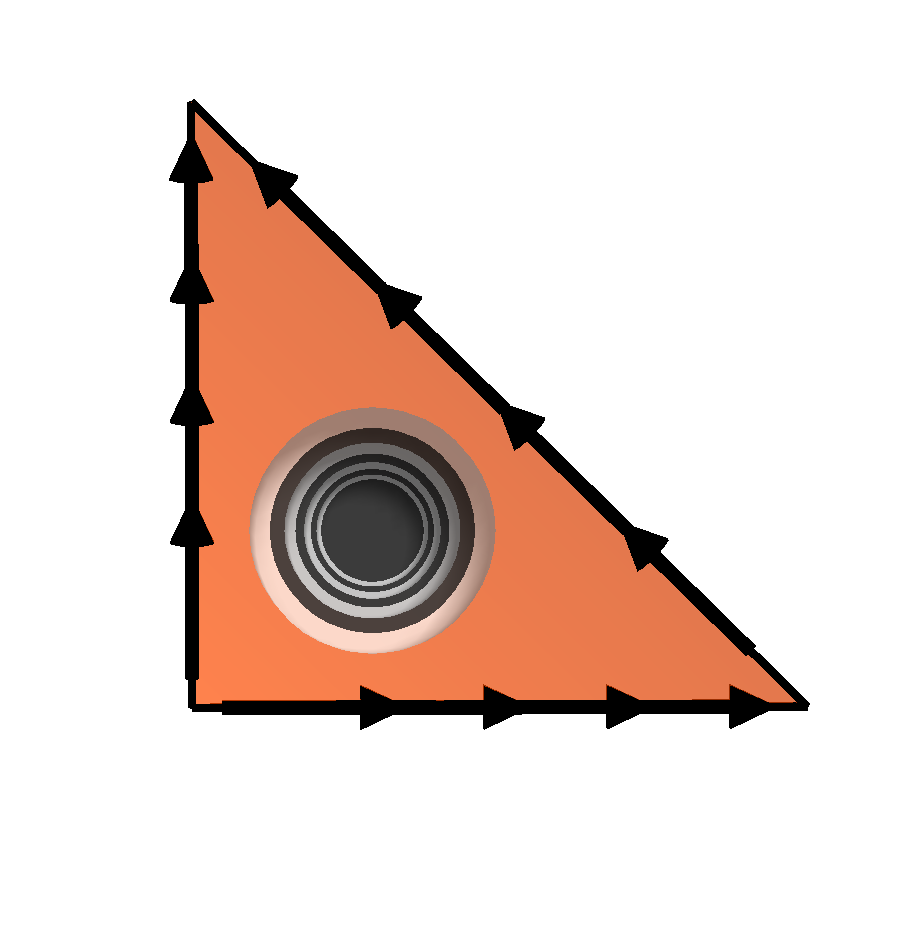
\includegraphics[width=1.3cm]{png/NED2_3_2d.png}
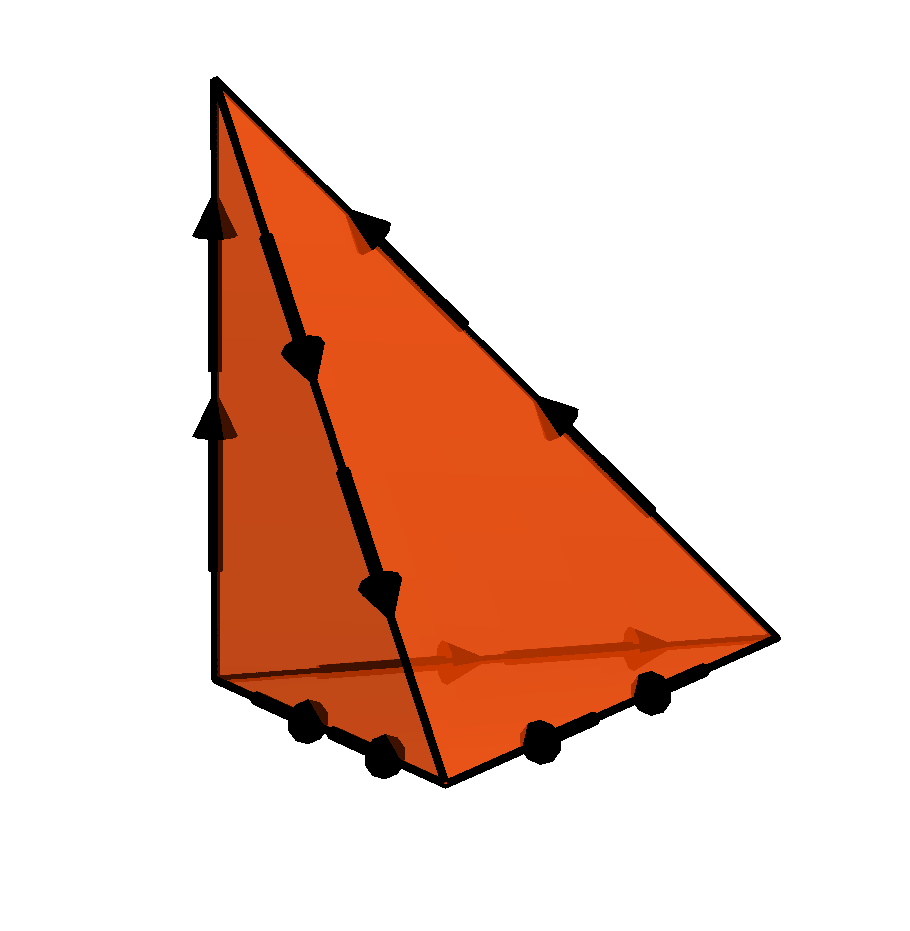
\includegraphics[width=1.3cm]{png/NED2_1_3d.png} \\
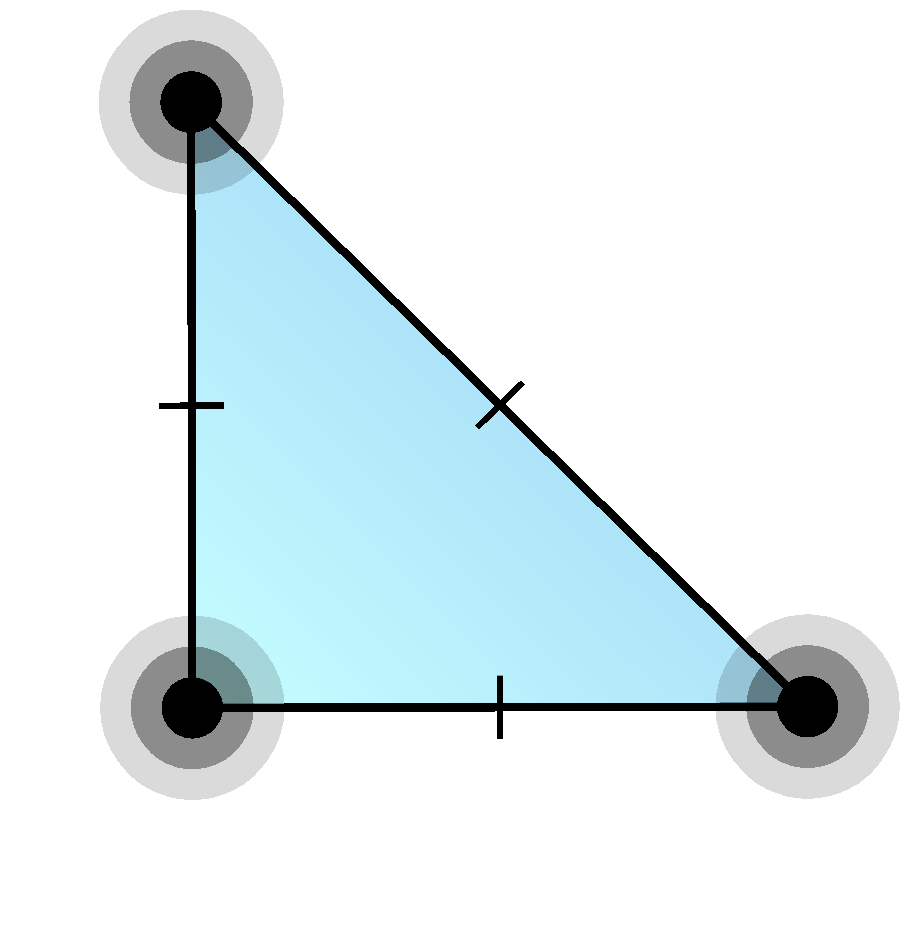
\includegraphics[width=1.3cm]{png/ARG5_2d.png}
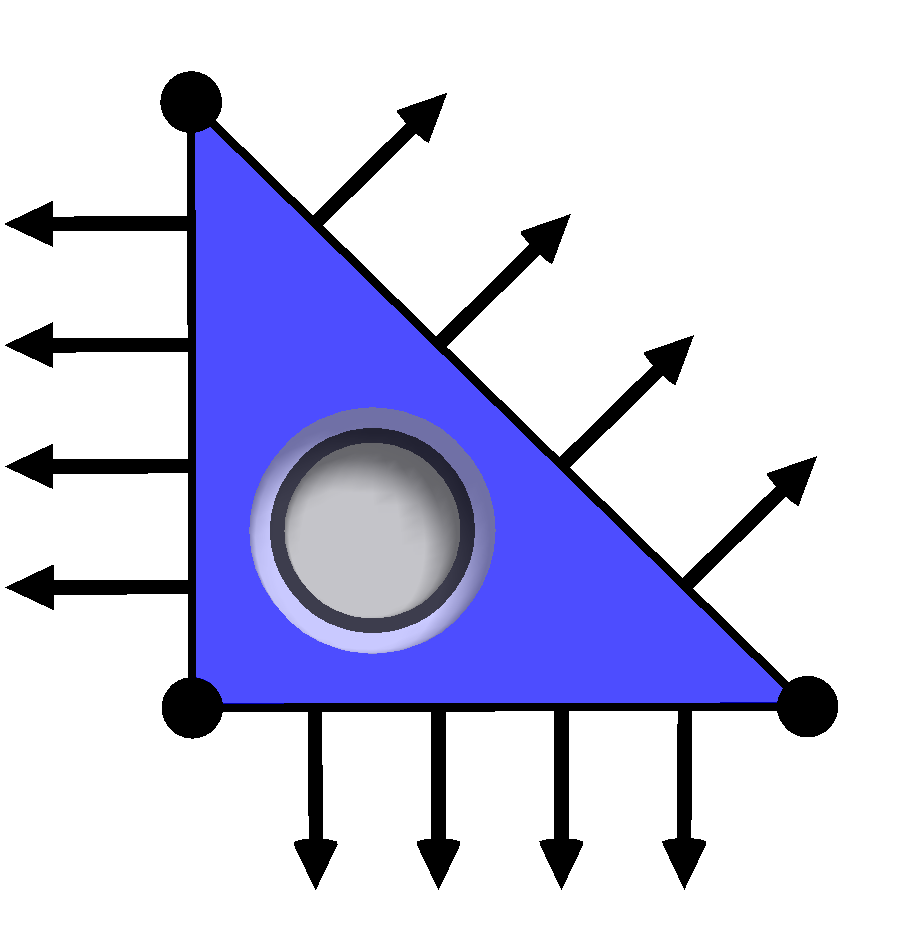
\includegraphics[width=1.3cm]{png/AW_2d.png}
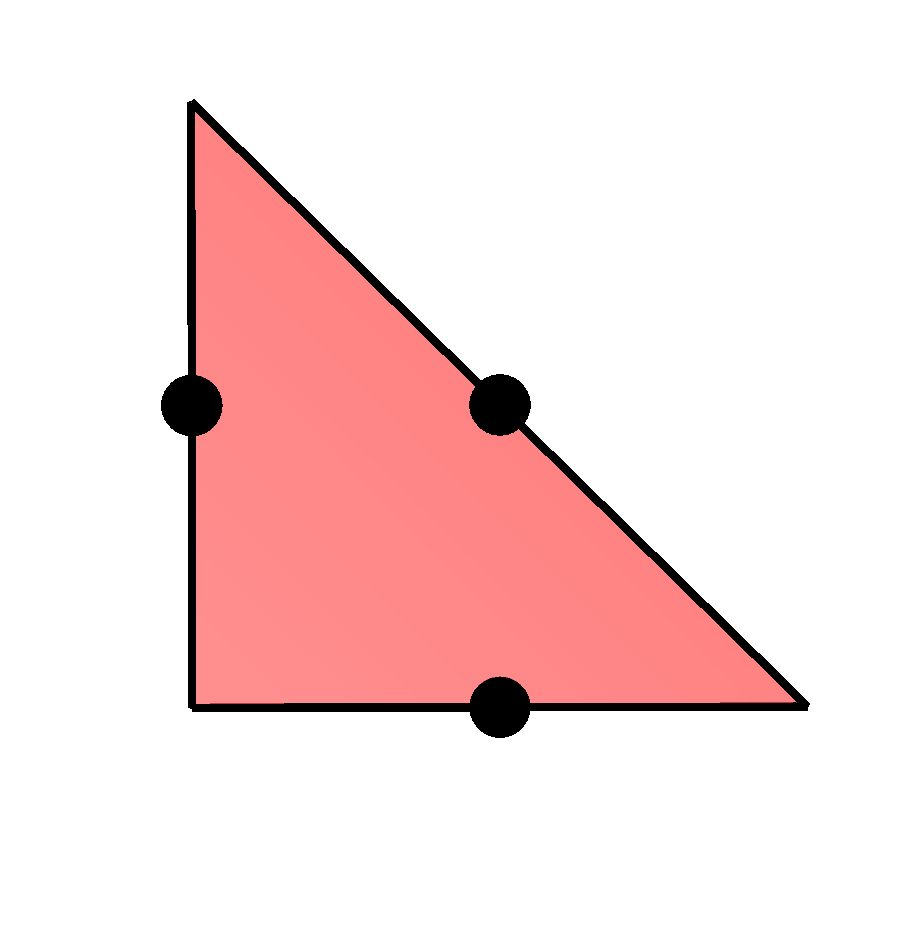
\includegraphics[width=1.3cm]{png/CR1_2d.png}
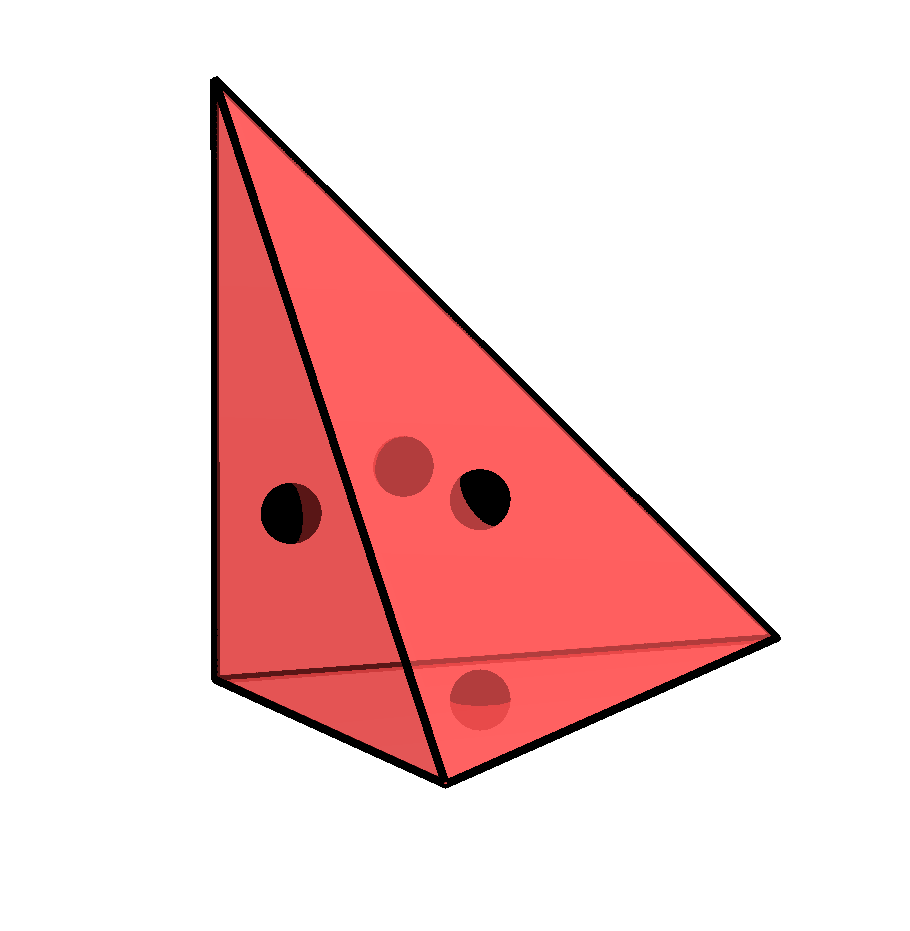
\includegraphics[width=1.3cm]{png/CR1_3d.png}
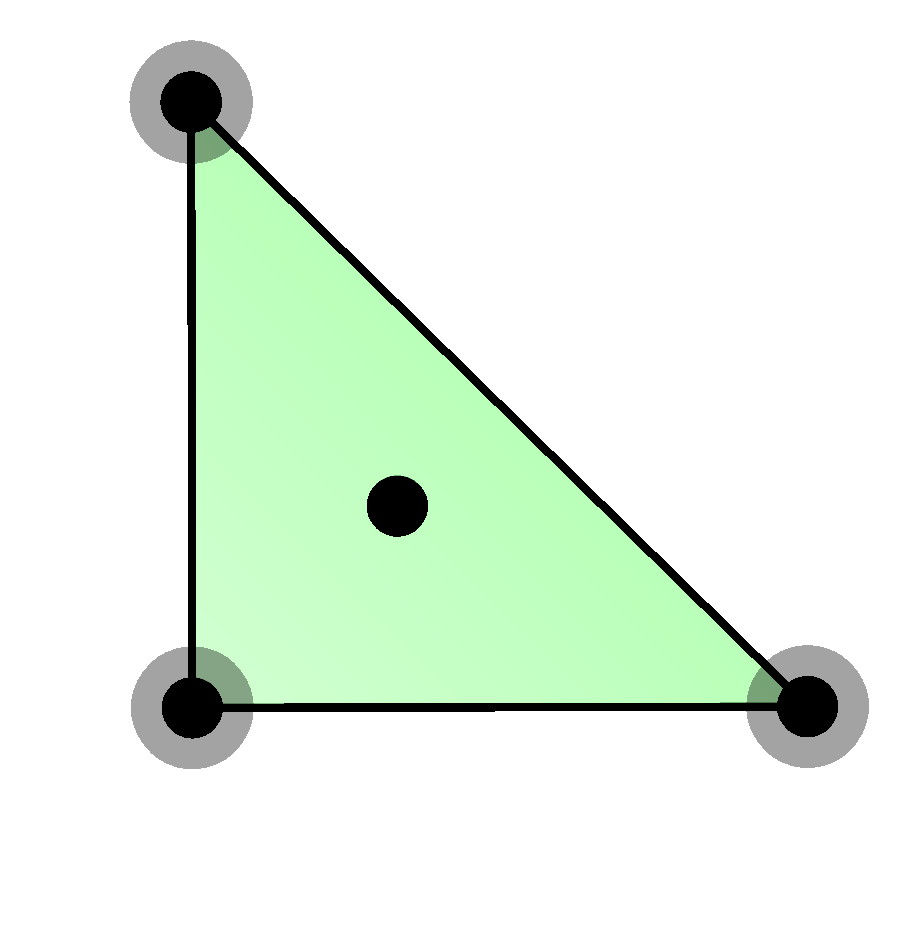
\includegraphics[width=1.3cm]{png/HER_2d.png}
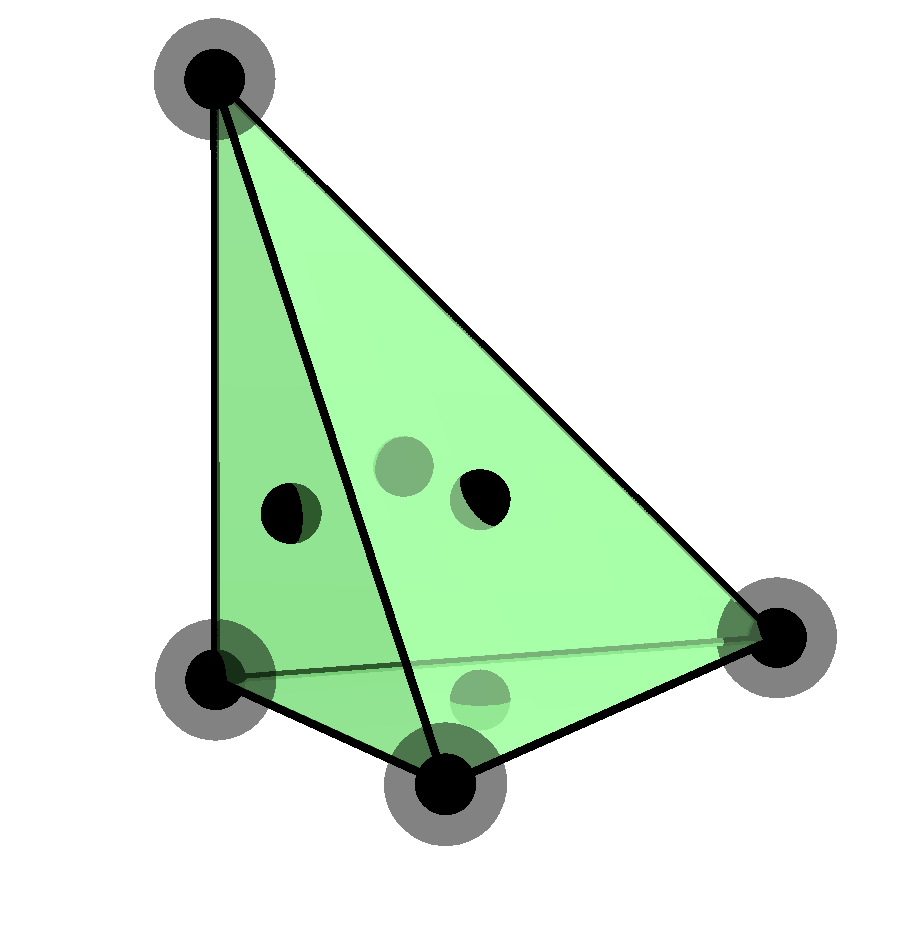
\includegraphics[width=1.3cm]{png/HER_3d.png}
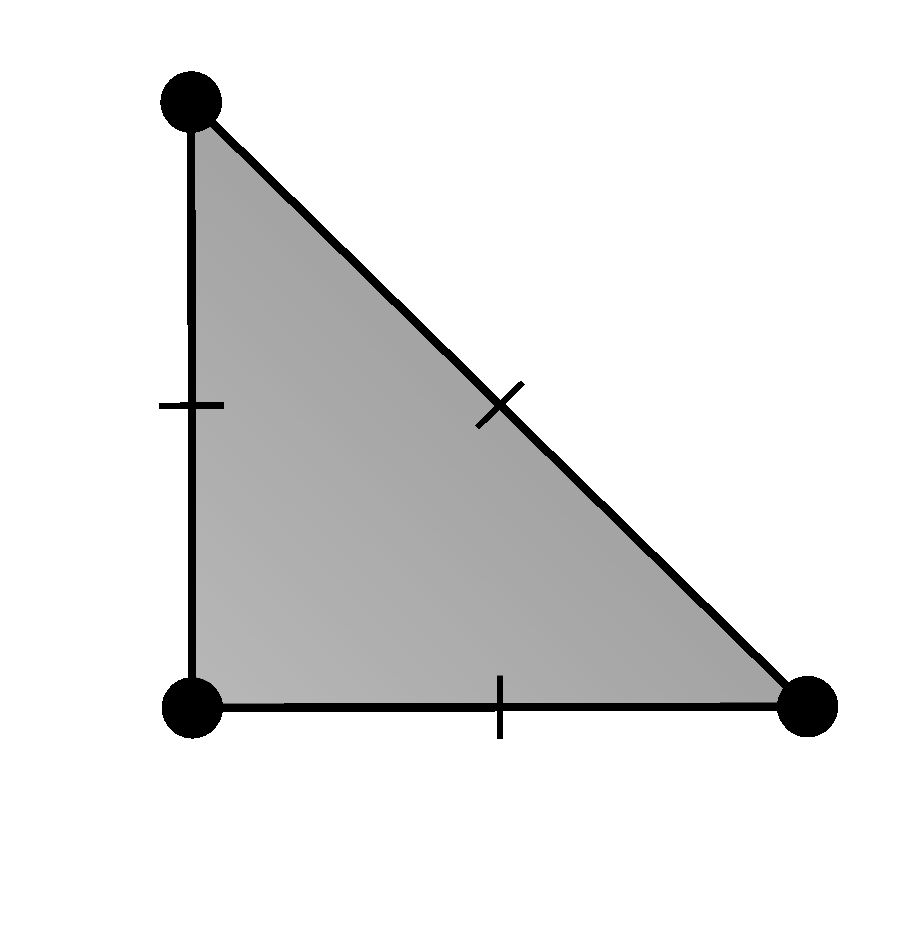
\includegraphics[width=1.3cm]{png/MOR_2d.png}
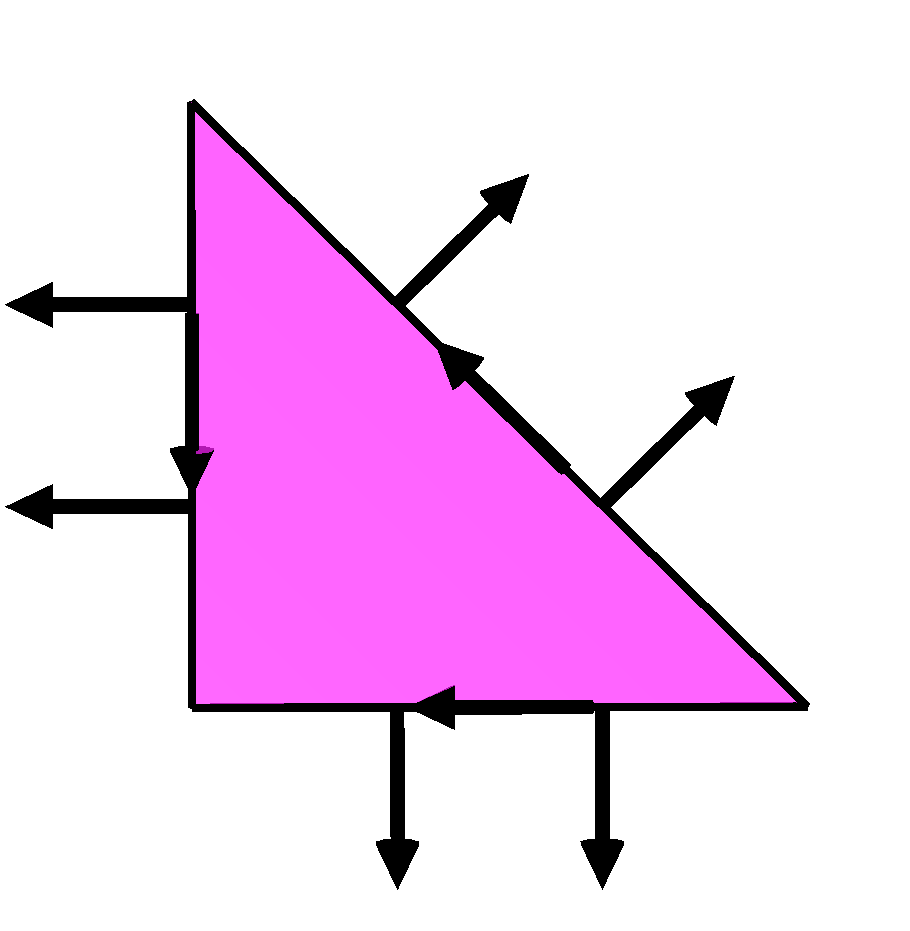
\includegraphics[width=1.3cm]{png/MTW_2d.png}

\end{frame}


\fenicssection{What has FEniCS been used for?}

\begin{frame}[fragile]
  \frametitle{Computational hemodynamics}

  \begin{center}
    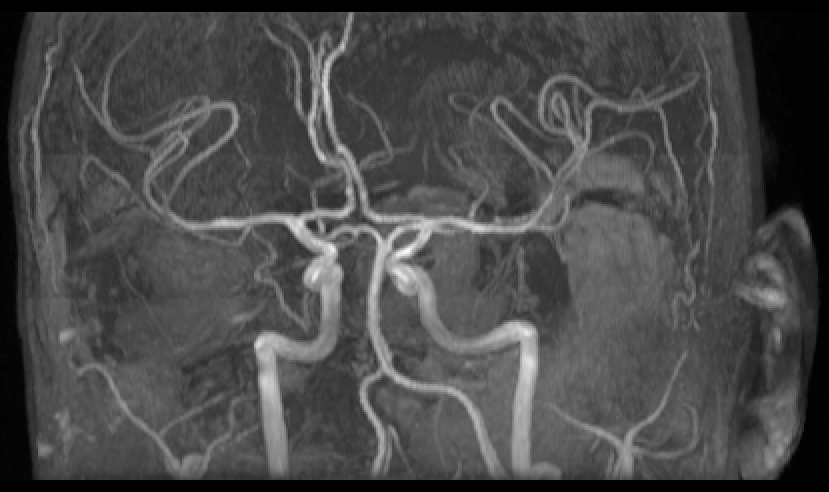
\includegraphics[height=3.5cm]{png/circle_of_willis_scan.png} \hspace{0.3cm}
    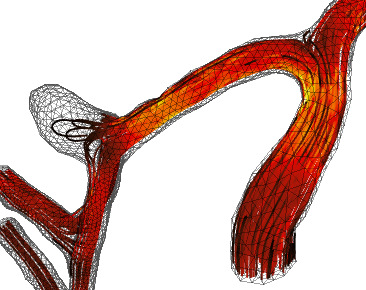
\includegraphics[height=3.5cm]{png/circle_of_willis_aneurysm.png}
  \end{center}

  \begin{itemize}
  \item
    Low wall shear stress may trigger aneurysm growth
  \item
    Solve the incompressible Navier--Stokes equations on patient-specific geometries
    \begin{displaymath}
      \begin{split}
        \dot{u} + u \cdot \nabla u - \nabla \cdot \sigma(u, p) &= f \\
        \nabla \cdot u &= 0
      \end{split}
    \end{displaymath}
  \end{itemize}

  \reference{Valen-Sendstad, Mardal, Logg}
            {Computational hemodynamics}
            {2011}

\end{frame}

\begin{frame}[fragile, shrink=50]
  \frametitle{Computational hemodynamics (contd.)}

  \vspace{2cm}

  \begin{columns}

    \begin{column}{0.5\textwidth}
      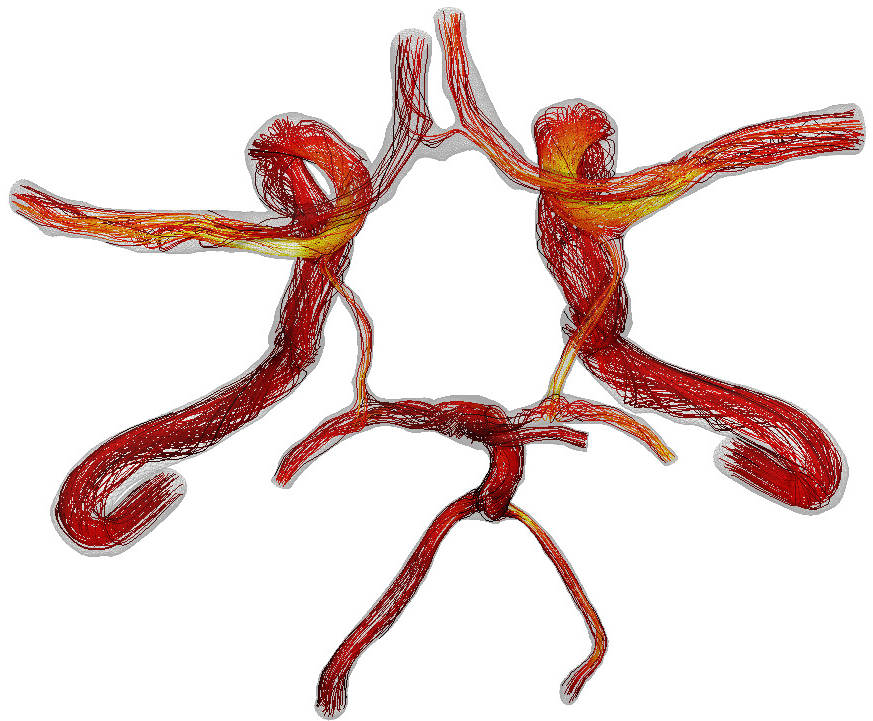
\includegraphics[width=\textwidth]{png/circle_of_willis_simulation.png}
    \end{column}

    \begin{column}{0.5\textwidth}
      \begin{python}
# Define Cauchy stress tensor
def sigma(v,w):
    return 2.0*mu*0.5*(grad(v) + grad(v).T)  - w*Identity(v.cell().d)

# Define symmetric gradient
def epsilon(v):
    return  0.5*(grad(v) + grad(v).T)

# Tentative velocity step (sigma formulation)
U = 0.5*(u0 + u)
F1 = rho*(1/k)*inner(v, u - u0)*dx + rho*inner(v, grad(u0)*(u0 - w))*dx \
   + inner(epsilon(v), sigma(U, p0))*dx \
   + inner(v, p0*n)*ds - mu*inner(grad(U).T*n, v)*ds \
   - inner(v, f)*dx
a1 = lhs(F1)
L1 = rhs(F1)

# Pressure correction
a2 = inner(grad(q), k*grad(p))*dx
L2 = inner(grad(q), k*grad(p0))*dx - q*div(u1)*dx

# Velocity correction
a3 = inner(v, u)*dx
L3 = inner(v, u1)*dx + inner(v, k*grad(p0 - p1))*dx
      \end{python}
    \end{column}

  \end{columns}

  % Compensate for scaling
  \huge

  \vspace{0.5cm}

  \begin{itemize}
  \item
    The Navier--Stokes solver is implemented in Python/FEniCS
  \item
    FEniCS allows solvers to be implemented in a minimal amount of code
  \end{itemize}

  \reference{Valen-Sendstad, Mardal, Logg}
            {Computational hemodynamics}
            {2011}

\end{frame}

\begin{frame}[fragile, shrink=50]
  \frametitle{Hyperelasticity}

  \vspace{1cm}

  \begin{columns}

    \begin{column}{0.5\textwidth}
      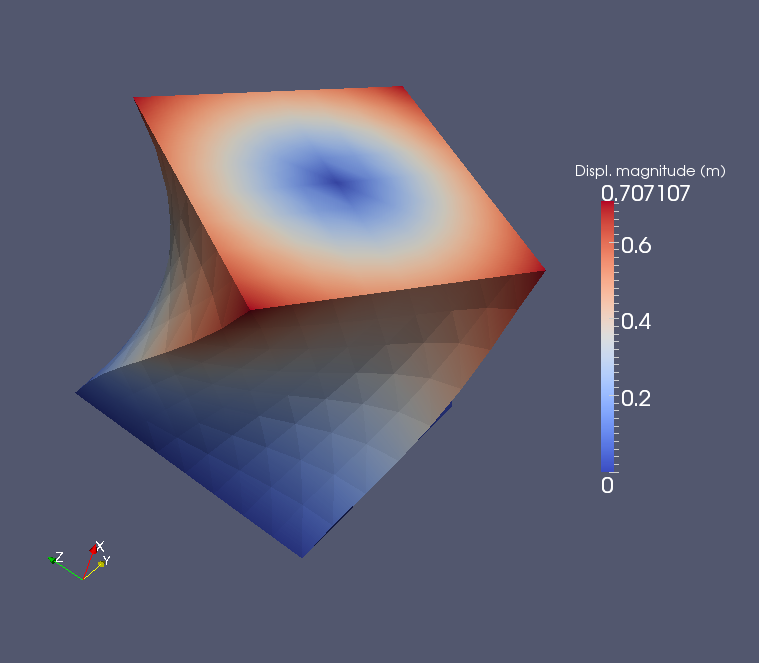
\includegraphics[width=\textwidth]{png/twistedcube.png}
    \end{column}

    \begin{column}{0.5\textwidth}
      \begin{python}
from fenics import *

mesh = UnitCubeMesh(24, 16, 16)
V = VectorFunctionSpace(mesh, "Lagrange", 1)

left =  CompiledSubDomain("(std::abs(x[0])       < DOLFIN_EPS) && on_boundary")
right = CompiledSubDomain("(std::abs(x[0] - 1.0) < DOLFIN_EPS) && on_boundary")

c = Expression(("0.0", "0.0", "0.0"), degree=0)
r = Expression(("0.0", 
"0.5*(y0+(x[1]-y0)*cos(t)-(x[2]-z0)*sin(t)-x[1])",
"0.5*(z0+(x[1]-y0)*sin(t)+(x[2]-z0)*cos(t)-x[2])"),
y0=0.5, z0=0.5, t=pi/3, degree=3)
bcl = DirichletBC(V, c, left)
bcr = DirichletBC(V, r, right)
bcs = [bcl, bcr]
v  = TestFunction(V)
u  = Function(V) 
B  = Constant((0.0, -0.5, 0.0))
T  = Constant((0.1,  0.0, 0.0))
I = Identity(V.cell().d)
F = I + grad(u)
Ic = tr(F.T*F)
J  = det(F)
E, nu = 10.0, 0.3
mu, lmbda = Constant(E/(2*(1 + nu))), Constant(E*nu/((1 + nu)*(1 - 2*nu)))
psi = (mu/2)*(Ic - 3) - mu*ln(J) + (lmbda/2)*(ln(J))**2
Pi = psi*dx - dot(B, u)*dx - dot(T, u)*ds
F = derivative(Pi, u, v)

solve(F == 0, u, bcs) 
plot(u, interactive=True, mode="displacement")
      \end{python}
    \end{column}
  \end{columns}

  % Compensate for scaling
  \huge

  \reference{H. Narayanan}
            {A computational framework for nonlinear elasticity}
            {2011}

\end{frame}


\fenicssection{How to use FEniCS?}
\begin{frame}
  \frametitle{Hello World in FEniCS: problem formulation}

  \begin{block}{Poisson's equation}
    \vspace{-0.5cm}
    \begin{displaymath}
      \begin{split}
        -\Delta u &= f \quad \mbox{ in } \Omega \\
        u &= 0 \quad \mbox { on } \partial\Omega
      \end{split}
    \end{displaymath}
  \end{block}

  \begin{block}{Finite element formulation}
    \vspace{1ex}
    Find $u \in V$ such that
    \begin{displaymath}
      \underbrace{\int_{\Omega} \nabla u \cdot \nabla v \dx}_{\textcolor{fenicsred}{a(u,v)}}
      = \underbrace{\int_{\Omega} f \, v \dx}_{\textcolor{fenicsred}{L(v)}}
      \quad \foralls v \in V
    \end{displaymath}
  \end{block}

\end{frame}

\begin{frame}[fragile]
  \frametitle{Hello World in FEniCS: implementation}

    \begin{python}
from fenics import *

mesh = UnitSquareMesh(32, 32)

V = FunctionSpace(mesh, "Lagrange", 1)
u = TrialFunction(V)
v = TestFunction(V)
f = Expression("x[0]*x[1]", degree=2)

a = dot(grad(u), grad(v))*dx
L = f*v*dx

bc = DirichletBC(V, 0.0, DomainBoundary())

u = Function(V)
solve(a == L, u, bc)
plot(u)
    \end{python}

\end{frame}

\begin{frame}
  \frametitle{Basic API}

  \begin{itemize}
  \item
    \texttt{Mesh},
    \texttt{Vertex},
    \texttt{Edge},
    \texttt{Face},
    \texttt{Facet},
    \texttt{Cell}
  \item
    \texttt{FiniteElement}, \texttt{FunctionSpace}
  \item
    \texttt{TrialFunction},
    \texttt{TestFunction},
    \texttt{Function}
  \item
    \texttt{grad()}, \texttt{curl()}, \texttt{div()}, \ldots
  \item
    \texttt{Matrix}, \texttt{Vector}, \texttt{KrylovSolver}, \texttt{LUSolver}
  \item
    \texttt{assemble()}, \texttt{solve()}, \texttt{plot()}
  \end{itemize}

  \vspace{1cm}

  \begin{itemize}
  \item
    Python interface generated semi-automatically by SWIG
  \item
    C++ and Python interfaces almost identical
  \end{itemize}

\end{frame}

\begin{frame}
    \frametitle{Sounds great, but how do I find my way through the
    jungle?}
    \begin{center}
        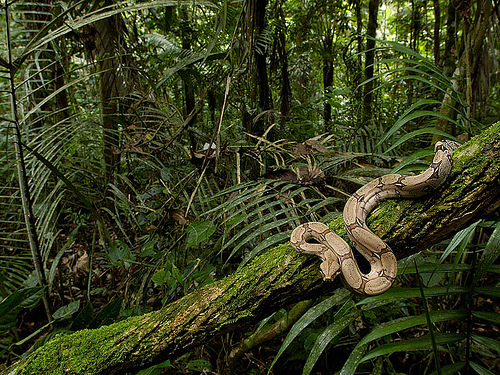
\includegraphics[width=0.8\textwidth]{jpg/jungle10.jpg}
    \end{center}
\end{frame}

\begin{frame}
    \frametitle{Three survival advices}
    \begin{columns}[c]
        \begin{column}{0.33\textwidth}
            \begin{center}
                
\includegraphics[width=0.99\textwidth]{png/python_logo.png}
            \end{center}
        \end{column}
        \begin{column}{0.33\textwidth}
            \begin{center}
                
\includegraphics[width=0.99\textwidth]{jpg/documentation.jpg}\\
            \end{center}
        \end{column}
        \begin{column}{0.33\textwidth}
            \begin{center}
                
\includegraphics[width=0.99\textwidth]{jpg/question-blue.jpg}
            \end{center}
        \end{column}
    \end{columns}
    \begin{columns}[t]
        \begin{column}{0.33\textwidth}
            \begin{center}
                \colemph{Use the right Python tools}
            \end{center}
        \end{column}
        \begin{column}{0.33\textwidth}
            \begin{center}
                \colemph{Explore the documentation}
            \end{center}
        \end{column}
        \begin{column}{0.33\textwidth}
            \begin{center}
                \colemph{Ask, report and request}
            \end{center}
        \end{column}
    \end{columns}
\end{frame}


\fenicssection{Use the right Python tools!}
\begin{frame}[shrink=10,t]
    \frametitle{Python tools}
    \begin{columns}[t]
        \begin{column}{0.45\textwidth}
            \begin{block}{Doc tools}
                \vspace{1em}
                \begin{itemize}
                    \item Standard terminal:
                        \\ \texttt{> pydoc dolfin}
                        \\ \texttt{> pydoc dolfin.Mesh}
                    \item Python console
                        \\ \texttt{>>> help(dolfin)}
                        \\ \texttt{>>> help(dolfin.Mesh)}
                \end{itemize}
            \end{block}
        \end{column}
        \begin{column}{0.60\textwidth}
    \begin{block}{Sophisticated Python environments}
        \begin{description}
            \item[IDLE] the official (but rather limited) Python IDE
            \item[IPython] \url{http://ipython.org/} provides a
                Python shell and notebook including syntax
                highlighting, tab-completion, object inspection,
                debug assisting, history \ldots
            \item[Eclipse] plugin \url{http://pydev.org/}
                includes syntax highlighting, code completion,
                unit-testing, refactoring, debugger \ldots
        \end{description}
    \end{block}
        \end{column}
    \end{columns}
\end{frame}

\begin{frame}
    \frametitle{IPython netbook}
    \begin{center}
        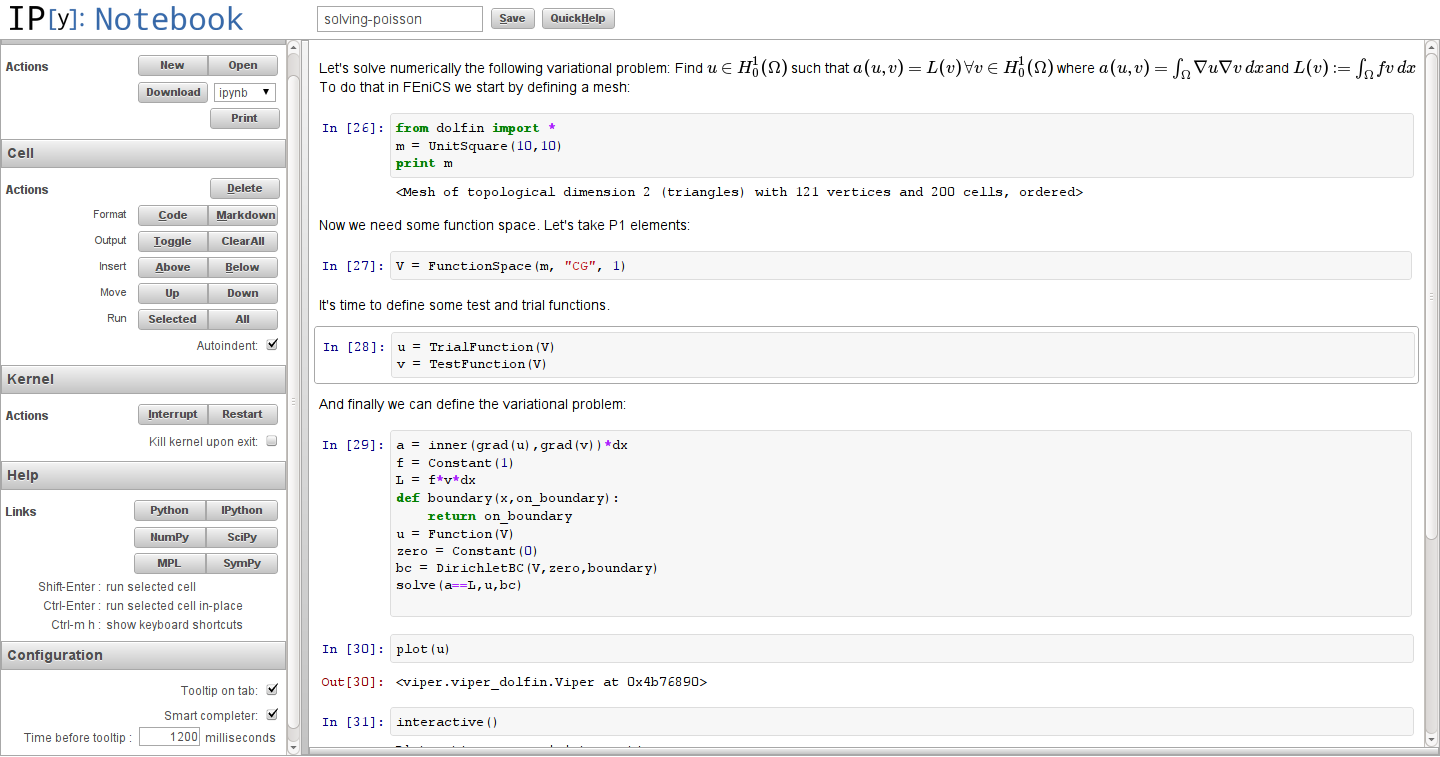
\includegraphics[width=0.90\textwidth,height=0.8\textheight]{png/solving-poisson-notebook}
%        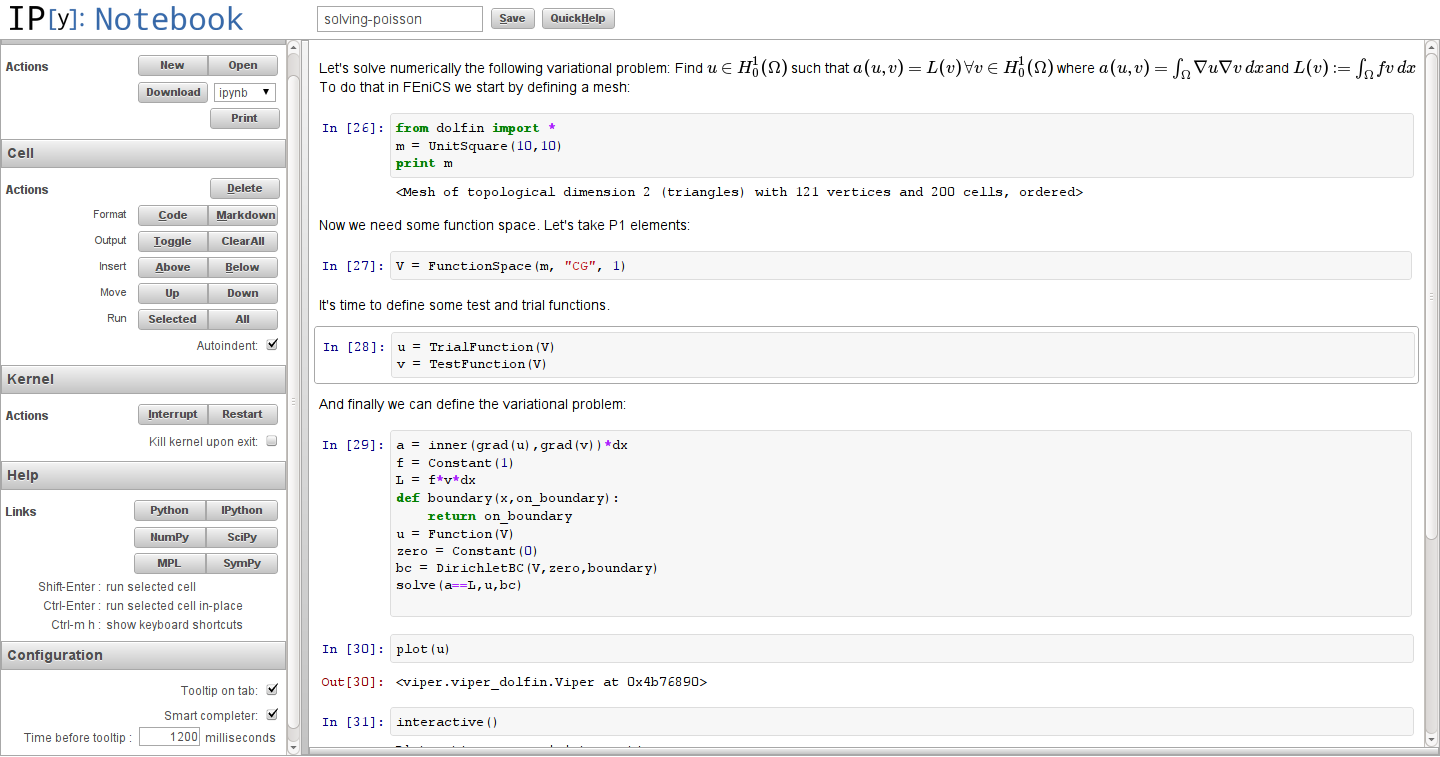
\includegraphics[width=0.99\textwidth]{png/solving-poisson-notebook.png}
%        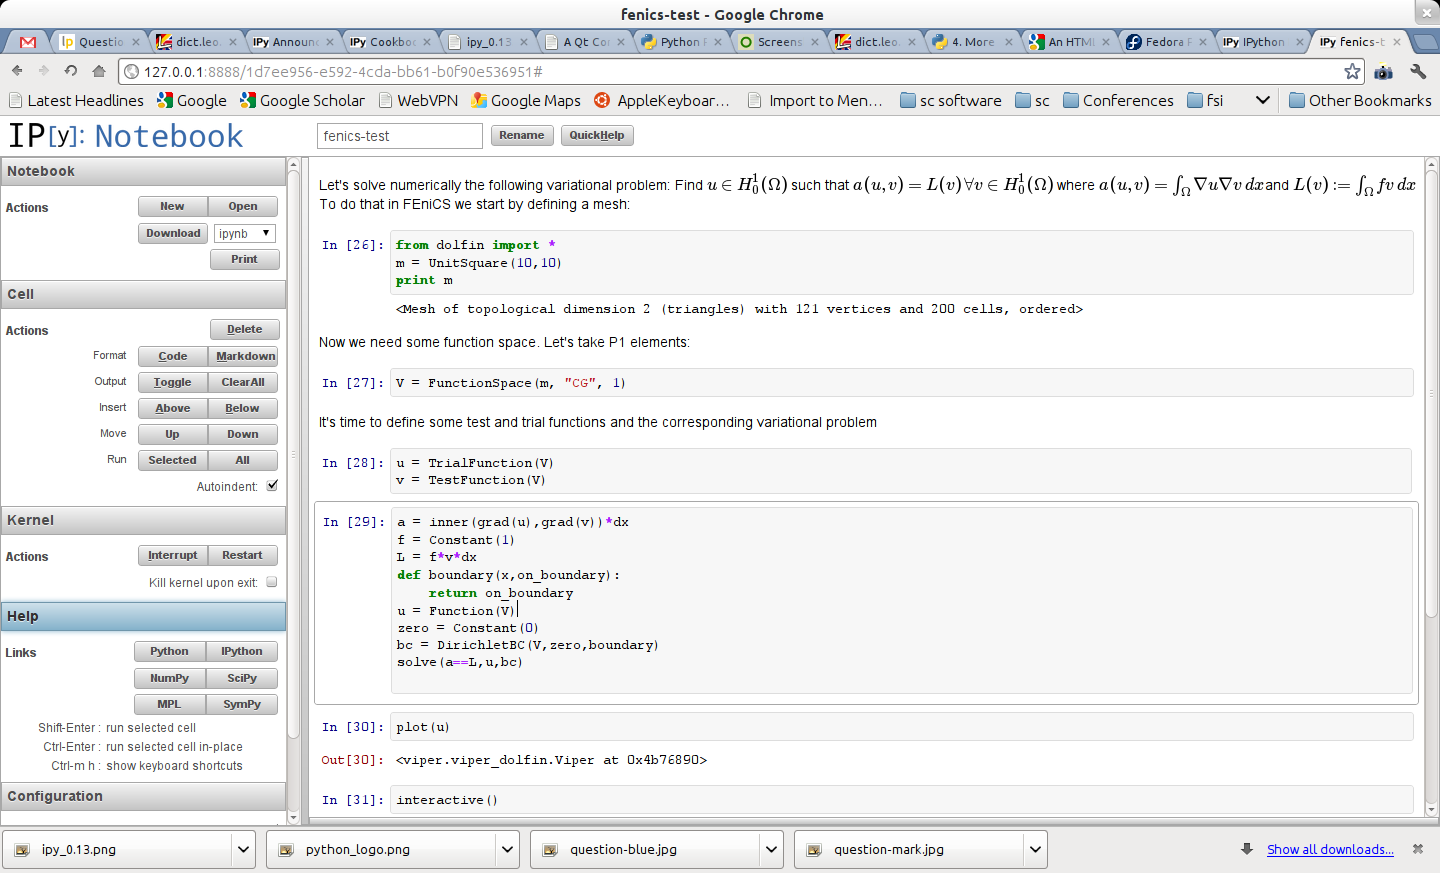
\includegraphics[width=0.90\textwidth,height=0.9\textheight]{png/fenics-in-ipython-netbook.png}
    \end{center}
\end{frame}

\begin{frame}
    \frametitle{Eclipse plugin Pydev}
    \begin{center}
        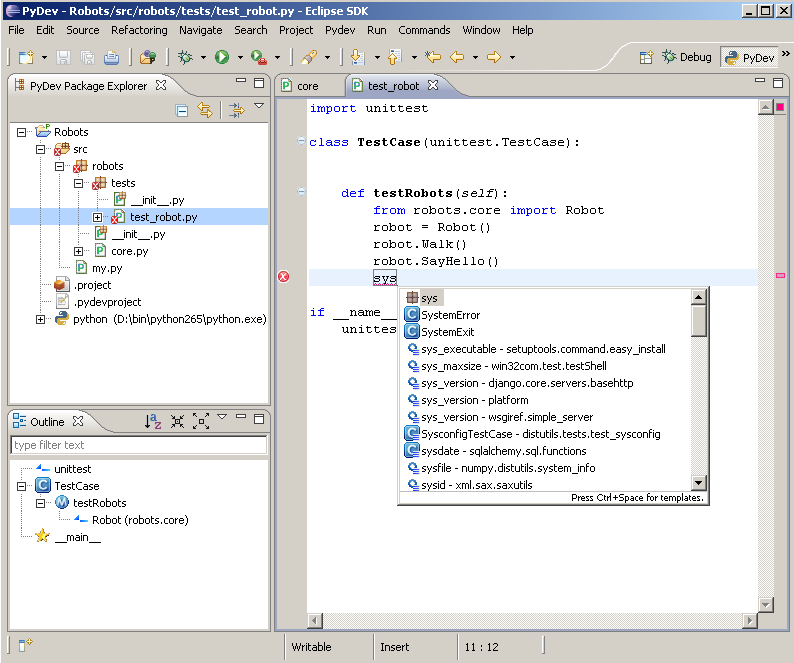
\includegraphics[height=0.9\textheight]{png/eclipse_screenshot_code_completion.png}
    \end{center}
\end{frame}

%\fenicssection{Use the documentation}
\fenicssection{Explore the FEniCS documentation!}
% TODO: Update webpage images when readthedocs work is completed

% Demos on old page
\begin{frame}
  \begin{center}
     {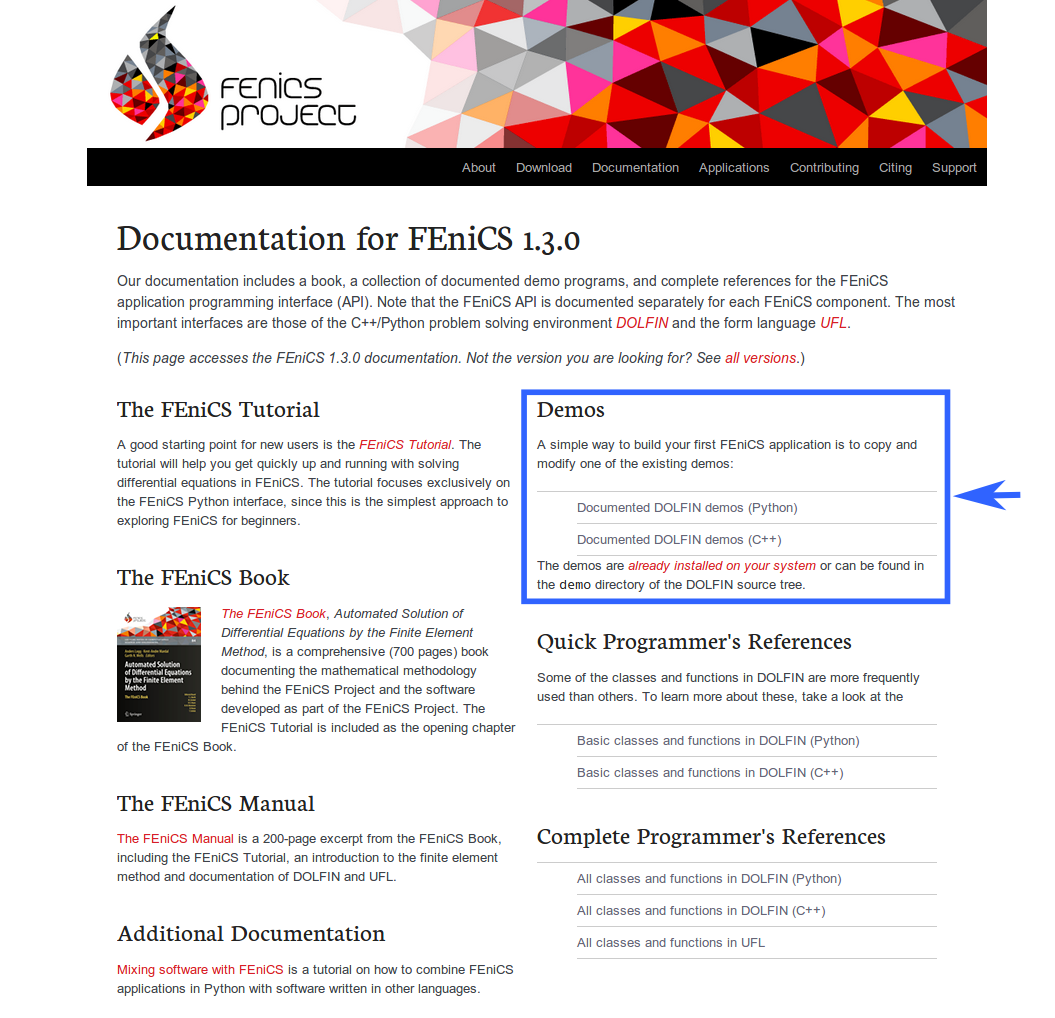
\includegraphics[width=0.80\textwidth]{png/fenics-doc-webpage-5.png}}
    \small
    \colemph{\url{http://fenicsproject.org/documentation/}}
  \end{center}
\end{frame}

% Reference docs on old page
\begin{frame}
  \begin{center}
     {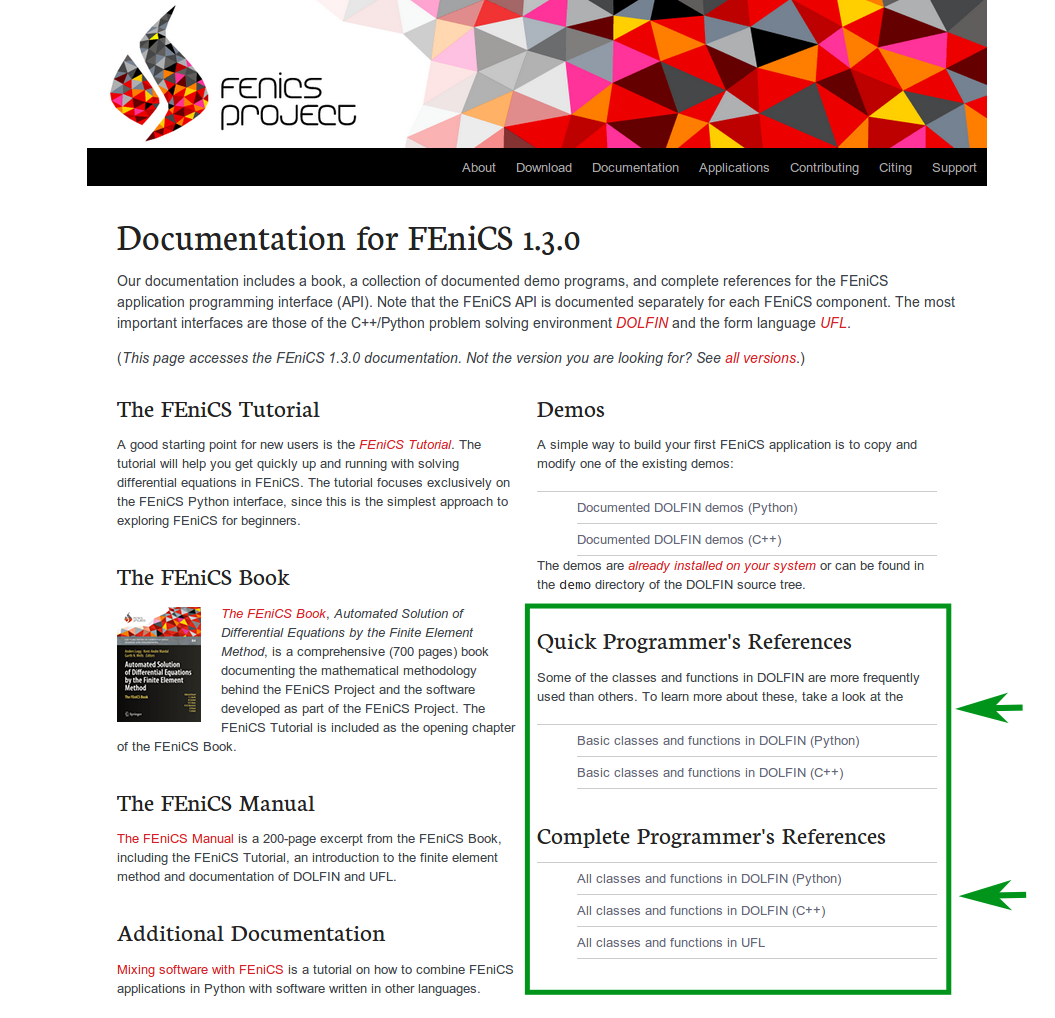
\includegraphics[width=0.80\textwidth]{png/fenics-doc-webpage-6.png}}
    \small
    \colemph{\url{http://fenicsproject.org/documentation/}}
  \end{center}
\end{frame}

% Currently migrating
\begin{frame}
  \begin{center}
     {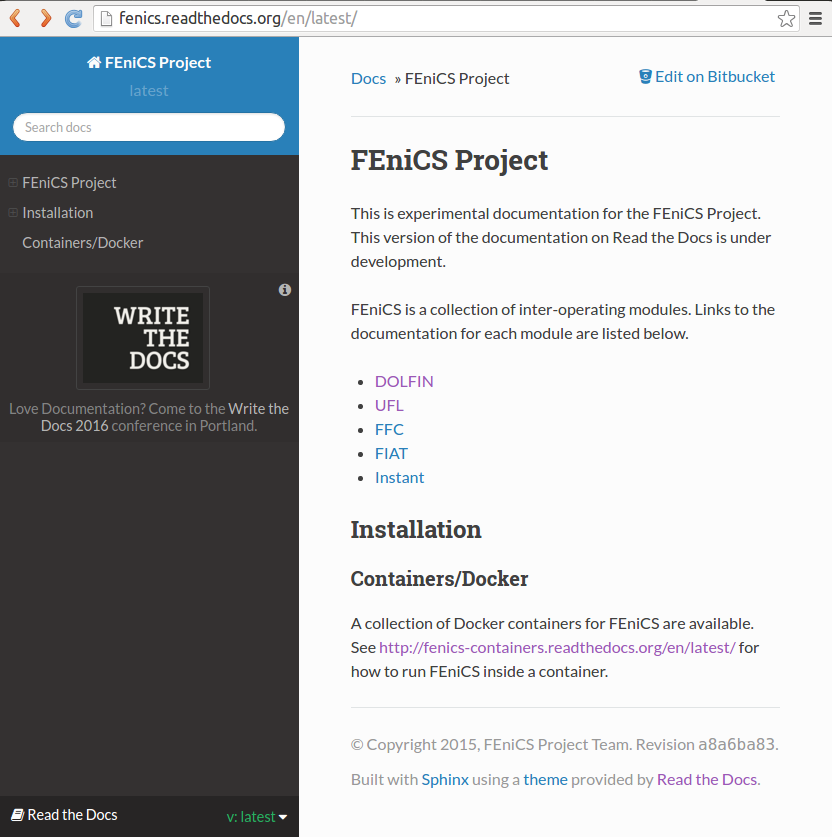
\includegraphics[width=0.80\textwidth]{png/fenics-readthedocs-webpage-1.png}}
    \small
    \colemph{\url{http://fenics.readthedocs.org/}}
  \end{center}
\end{frame}

\fenicssection{Ask questions, report bugs and request new features!}
\begin{frame}
    \frametitle{Development community is organized via bitbucket.org}
    \begin{center}
        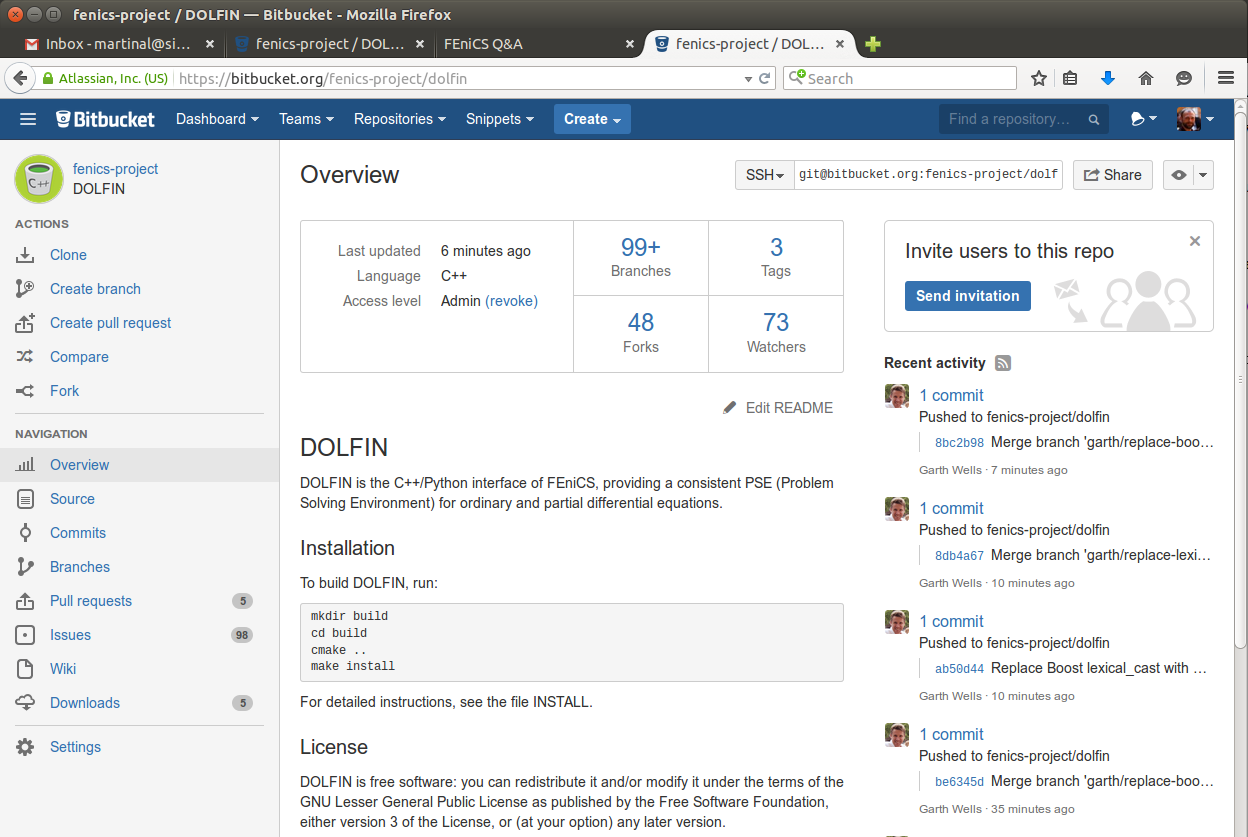
\includegraphics[height=0.75\textheight]{png/fenics-bitbucket-webpage.png}
        \vspace{1em}
        \small
        \colemph{\url{http://bitbucket.org/fenics-project/}}
    \end{center}
\end{frame}
\begin{frame}
    \frametitle{Community help is available via QA forum}
    \begin{center}
        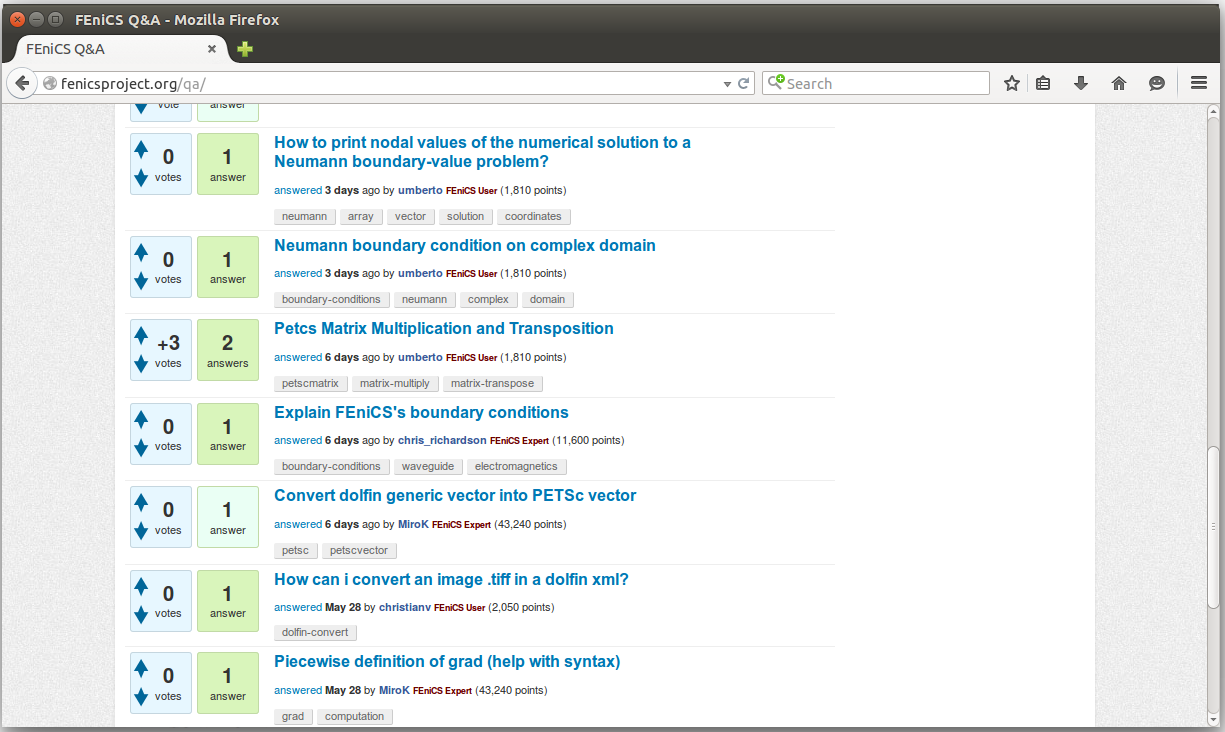
\includegraphics[width=1.0\textwidth,height=0.7\textheight]{png/fenics-qa-website.png}
        \vspace{1em}
        \small
        \colemph{\url{https://fenicsproject.org/qa}}
    \end{center}
\end{frame}


\begin{frame}
  \frametitle{Installation alternatives}

  % FEniCS uses standard setup.py and cmake tools
  % but dependencies are tricky to configure.

  \begin{tabular}{cp{10cm}}
    \includegraphics[height=1cm]{png/docker_logo.png} &
    \begin{minipage}{10cm}
      \ding{43} Docker images on Linux, Mac, Windows
      \vspace{0.6cm}
    \end{minipage}
    \\
    \includegraphics[height=1cm]{png/source.png} &
    \begin{minipage}{10cm}
      \ding{43} Build from source with Hashdist (fenics-install.sh)
      \vspace{0.8cm}
    \end{minipage}
    \\
    \includegraphics[height=1cm]{png/ubuntu_logo.png} &
    \begin{minipage}{10cm}
      \ding{43} PPA with apt packages for Debian and Ubuntu
      \vspace{0.6cm}
    \end{minipage}
    \\
    \includegraphics[height=1cm]{png/mac_osx_logo.png} &
    \begin{minipage}{10cm}
      \ding{43} Drag and drop installation on Mac OS X
      \vspace{0.8cm}
    \end{minipage}
  \end{tabular}

  \begin{center}
    \colemph{\url{http://fenicsproject.org/download/}}
  \end{center}

\end{frame}

\begin{frame}
  \frametitle{\emph{The FEniCS challenge!}}
 \begin{center}
      \begin{enumerate}
          \item Install FEniCS on your laptop!
              \\
              \vspace{1em}
              \colemph{\url{http://fenicsproject.org/download/}}
              \vspace{1em}
            \item Find and execute \texttt{demo\_cahn-hilliard.py},
              try to visualize the results with Paraview.
          \item What are the main packages of the \texttt{dolfin}
              module?
          \item Which elements are supported in \texttt{dolfin}?
          \item Plot at least two finite elements from each row on page 4
              and identify those elements you are most curious about!
      \end{enumerate}
  \end{center}
\end{frame}


\end{document}
